\documentclass[a4paper]{article}
% Add "final" option in the article to remove todo
\usepackage[common_math_textnormal,todonotes,math_base_note,math_simple]{gatmeo}
\usepackage{ytableau}
\usepackage{CJKutf8}
\usepackage{tikz-cd}
%\doublespacing
\newcommand{\mathintitle}[1]{\texorpdfstring{$#1$}{\detokenize{#1}}}

\title{\bf{
        The Bicharacteristic Polynomial of the Type A Springer Resolution
}}

\newcommand{\ansonlaw}{\FirstBigRestSmallCaps{Sum kiu Law}\thanks{sklaw@math.cuhk.edu.hk}}
\renewcommand{\omegat}{\FirstBigRestSmallCaps{Nok to Omega Tong}\thanks{onttong@math.cuhk.edu.hk}}
%\author{\ansonlaw\thanks{
%  Department of Mathematics, The Chinese University of Hong Kong. The author has been an MPhil student since September 2023. He is expected to graduate in the summer of 2025.
%}, \omegat\thanks{
%  Department of Mathematics, The Chinese University of Hong Kong. The author has been an MPhil student since September 2023. He is expected to graduate in the summer of 2025.
%}}
\author{\ansonlaw\ {\small{AND}} \omegat\\\\
\emph{Department of Mathematics, The Chinese University of Hong Kong, Hong Kong}
}
\date{}
%sklaw@math.cuhk.edu.hk, onttong@math.cuhk.edu.hk\\\\

\newcommand{\noskipline}{\vspace{-1.5em}}

\newcommand{\II}{\mathcal{I}}
\newcommand{\BB}{\mathcal{B}}

\renewcommand{\epsilon}{\varepsilon}
\renewcommand{\phi}{\varphi}
\newcommand{\NN}{\mathcal{N}}
\newcommand{\OO}{\mathcal{O}}
\newcommand{\ZZ}{\mathbb{Z}}
\tikzcdset{
    cells={font=\everymath\expandafter{\the\everymath\displaystyle}},
}

% Hypertoric Variety
\newcommand{\MM}{\mathcal{M}}
\newcommandx*\Mper[1][1=\Gamma]{\mathcal{M}^{\mathrm{per}}(#1)}
\newcommandx*\Mperchar[2][2=\Gamma]{\mathcal{M}^{\mathrm{per}}_{#1}(#2)}
\newcommandx*\Hper[1][1=\Gamma]{\mathcal{A}^{\mathrm{per}}(#1)}
\newcommandx*\Hperchar[2][2=\Gamma]{\mathcal{A}^{\mathrm{per}}_{#1}(#2)}
\newcommandx*\Rper[2][1=\bullet, 2=\Gamma]{\mathcal{R}_{\mathrm{per}}^{#1}(#2)}
\newcommandx*\SRper[2][1=\bullet, 2=\Gamma]{\mathcal{SR}_{\mathrm{per}}^{#1}(#2)}
\newcommandx*\Mfin[1][1=\Gamma]{\mathcal{M}(#1)}
\newcommandx*\Mfinchar[2][2=\Gamma]{\mathcal{M}_{#1}(#2)}
\newcommandx*\Hfinchar[2][2=\Gamma]{\mathcal{A}_{#1}(#2)}
\newcommandx*\Hfin[1][1=\Gamma]{\mathcal{A}(#1)}
\newcommandx*\Rfin[2][1=\bullet, 2=\Gamma]{\mathcal{R}^{#1}(#2)}
\newcommandx*\SR[2][1=\bullet, 2=\Gamma]{\mathcal{SR}^{#1}(#2)}
\newcommandx*\Mmul[1][1=\Gamma]{\mathcal{M}^{\mathrm{mul}}(#1)}
\newcommandx*\idealIper[1][1=\Gamma]{I_{\mathrm{per}}(#1)}
\newcommandx*\idealI[1][1=\Gamma]{I(#1)}
\newcommand{\opendisc}{\mathbb{D}}
\newcommandx*\Betti[1][1=\Gamma]{\mathfrak{B}(#1)}
\newcommandx*\Dolbeault[1][1=\Gamma]{\mathfrak{D}(#1)}

% Core and Toric
\newcommandx*\corefin[1][1=\Gamma]{\mathcal{L}(#1)}
\newcommandx*\coreper[1][1=\Gamma]{\mathcal{L}^{\mathrm{per}}(#1)}
\newcommandx*\toricP[1][1=P]{\mathcal{X}(#1)}
\newcommandx*\fixptP[1][1=B]{P_{#1}}
\newcommandx*\toricB[1][1=B]{\mathcal{X}(#1)}

% Complex
% Group Cohomology Complex
\newcommand{\pGC}{\mathfrak{C}} 
\newcommandx*\GC[3][1=\bullet,2=\bullet,3=\Gamma]{\mathfrak{C}^{#1,#2}(#3)} % Our complex: Group Cohomology
\newcommand{\dGC}{\delta} % Our complex: Group Cohomology
\newcommand{\dGCbar}{\bar{\delta}} % Our complex: Group Cohomology
\newcommand{\fGC}{\phi}
\newcommand{\gGC}{\psi}
\newcommand{\hGC}{\eta}
%--- Group Cohomology Complex with e
\newcommandx*\GCe[4][1=\bullet,2=\bullet,3=\Gamma,4=e]{\mathfrak{C}^{#1,#2}(#3,#4)}
\newcommand{\dGCe}{\delta_e}
\newcommand{\fGCe}{\mathfrak{f}}
\newcommand{\gGCe}{\mathfrak{g}}
\newcommand{\hGCe}{\mathfrak{h}}
%--- CKS
\newcommandx*\GCS[2][1=\bullet,2={\Gamma, S}]{\mathfrak{D}^{#1}(#2)}
\newcommandx*\dGCS[1][1=S]{\dGC_{#1}}
\newcommandx*\fGCS[1][1=S]{\fGC_{#1}}
\newcommandx*\gGCS[1][1=S]{\gGC_{#1}}
\newcommandx*\hGCS[1][1=S]{\hGC_{#1}}
\newcommandx*\CKS[4][1=\bullet,2=\bullet,3=\bullet,4=\Gamma]{\mathfrak{C}^{#1,#2,#3}(#4)} % CKS
\newcommandx*\grCKS[4][1=\bullet,2=\bullet,3=\bullet,4=\Gamma]{I^{#1, #2}\mathfrak{C}^{#3}(#4)} % CKS
\newcommandx*\CKSdiffgrading[3][1=\bullet,2=\bullet,3=\Gamma]{\mathfrak{C}'^{#1,#2}(#3)} % CKS
\newcommand{\dCKS}{d} %CKS Complex
\newcommand{\fCKS}{f}
\newcommand{\gCKS}{g}
\newcommand{\hCKS}{h}
\newcommandx*\HT[3][1=\bullet,2=\bullet,3=\Gamma]{\mathfrak{K}_{\mathrm{per}}^{#1, #2}(#3)}
\newcommandx*\grHT[3][1=\bullet,2=\bullet,3=\Gamma]{I^{#1}\mathfrak{K}_{\mathrm{per}}^{#2}(#3)}
\newcommand{\dHT}{\dCKS_{\mathrm{per}}}
\newcommandx*\HTalt[2][1=\bullet,2=\Gamma]{\tilde{\mathfrak{K}}^{#1}(#2)}
\newcommand{\dHTalt}{\tilde{\dCKS}_{\mathrm{per}}}
\newcommand{\fHT}{\fCKS_{\mathrm{per}}}
\newcommand{\gHT}{\gCKS_{\mathrm{per}}}
\newcommand{\hHT}{\hCKS_{\mathrm{per}}}
\newcommandx*\HTfin[3][1=\bullet,2=\bullet,3=\Gamma]{\mathfrak{K}^{#1, #2}(#3)}
\newcommandx*\grHTfin[3][1=\bullet,2=\bullet,3=\Gamma]{I^{#1}\mathfrak{K}^{#2}(#3)}
\newcommand{\dHTfin}{\dCKS}
\newcommand{\fHTfin}{\fCKS}
\newcommand{\gHTfin}{\gCKS}
\newcommand{\hHTfin}{\hCKS}
\newcommandx*\CPX[3][1=\bullet,2=\bullet,3=\Gamma]{\mathfrak{D}^{#1,#2}(#3)} % Intermediate complex
\newcommandx*\euler[3][3=\Gamma]{\eta^{#1, #2}(#3)}

% Graph and Matroids
% \newcommandx*\Tutte[2][1=\Gamma]{T(#1;\, #2)}
\newcommandx*\hpoly[2][1=\Gamma]{h(#1;\, #2)}
\newcommandx*\HTutte[2][1=\Gamma]{H(#1;\, #2)}
\newcommandx*\seqn[1][1=n]{[-#1,#1]}
\newcommand{\loopgraph}{{\bigcirc\!\!\bullet}}
\newcommand{\bridgegraph}{{\bullet\mspace{-7mu}-\mspace{-7mu}\bullet}}
\newcommand{\supnorm}[1]{\| #1 \|_{\infty}} 

\newcommand{\del}{\setminus}
\newcommand{\con}{\mathbin{/}}
\newcommand{\Gammaper}{\Gamma_{\mathrm{per}}}
\newcommandx*\tree[2][2=\Gamma]{\mathcal{T}_{#2}(#1)}
\newcommandx*\treefunction[1][1=\Gamma]{\mathcal{T}_{#1}}
\newcommandx*\cotreefunction[1][1=\Gamma]{\mathcal{T}_{#1}^*}
\newcommandx*\cotree[2][2=\Gamma]{\mathcal{T}_{#2}^*(#1)}
\newcommandx*\face[2][1=\bullet,2=\Gamma]{F_{#1}(#2)}
\newcommandx*\faceshelling[3][2=\bullet,3=\Gamma]{F_{#2}^{(#1)}(#3)}
\newcommandx*\faceper[2][1=\bullet,2=\Gamma]{F^{\mathrm{per}}_{#1}(#2)}
\newcommandx*\pair[3][3=\Gamma]{\langle #1, #2 \rangle_{#3}}
\newcommandx*\cotreein[2][2=\Gamma]{\mathcal{D}_{#2}(#1)}
\newcommandx*\cotreeinper[2][2=\Gamma]{\mathcal{D}^\per_{#2}(#1)}
\newcommandx*\cotreeinfunction[1][1=\Gamma]{\mathcal{D}_{#1}}
\newcommandx*\externalactivity[2][2=\Gamma]{EA_{#2}(#1)}
\newcommandx*\internalactivity[2][2=\Gamma]{IA_{#2}(#1)}
\newcommand{\intp}[1]{\iota_{#1}} % interior product
\newcommandx*\fundcycle[2][2=\Gamma]{\gamma_{#1}}
\newcommandx*\fundcyclewithtree[2][2=B]{\gamma_{#2,#1}}
\newcommandx*\fundbond[2][2=\Gamma]{\beta_{#1}}
\newcommandx*\fundbondwithtree[2][2=B]{\beta_{#2^*,#1}}
\newcommandx*\basis[2][1=\bullet,2=\Gamma]{\mathcal{B}_{#1}(#2)}
\newcommandx*\basisper[2][1=\bullet,2=\Gamma]{\mathcal{B}^\per_{#1}(#2)}

\newcommandx*\SE[3][1=,3=]{
  \ifstrempty{#3}
  {\ifstrempty{#1}{E^\bullet_{#2}}{#1_{#2}}}
  {\ifstrempty{#1}{E_{#2}(#3)}{#1_{#2}}}
}
\newcommandx*\HMGZ[2][1=\Gamma,2=\bullet]{H^{#2}(\MM(#1),\mathbb{Z})}
\newcommand{\hCCC}{\hat{\mathfrak{C}}}

\newcommand{\per}{\mathrm{per}}

% Math Operations
\newcommand{\HH}{\mathrm{H}}
\newcommand{\IH}{\mathrm{IH}}
\newcommandx*\Ext[1][1=\bullet]{\bigwedge\nolimits^{#1}}
\newcommandx*\Sym[1][1=\bullet]{\mathrm{Sym}^{#1}}
\newcommand{\sgn}{\mathrm{sgn}}
\newcommand{\coker}{\operatorname{coker}}
\renewcommand{\im}{\operatorname{im}}
\newcommand{\supp}{\mathrm{supp}}
\newcommand{\Hom}{\mathrm{Hom}}

% Group Cohomology
\newcommand{\invar}[1]{\Gamma_{#1}}
\newcommandx*\Rder[1][1=\bullet]{R^{#1}}
\newcommandx*\totRder[1][1=\bullet]{\mathbb{R}^{#1}}

% Homotopy Equivalence
\newcommand{\choice}[1]{[#1]} % choice for HTfin equiv
\newcommandx*\intord[2][2=S]{[#2]^{#1}} % integration order for GCS equiv
\newcommandx*\hyppl[2][2=S]{\alpha^{#2}_{#1}} % hyperplane for GCS equiv

\makeatletter
\newcommand{\GIT}[1][\@nil]{%
  \def\tmp{#1}%
  \ifx\tmp\@nnil
    /\!\!/%
  \else
    /\!\!/_{\! #1}%
  \fi
}
\newcommand{\HQ}[1][\@nil]{%
  \def\tmp{#1}%
  \ifx\tmp\@nnil
    /\!\!/\!\!/\!\!/%
  \else
    /\!\!/\!\!/\!\!/_{\! #1}%
  \fi
}
\makeatother

\newcommand{\Diff}{\mathrm{Diff}}
\newcommand{\Sympl}{\mathrm{Sympl}}
\newcommand{\acton}{\curvearrowright}
\newcommand{\smth}{C^\infty}
\newcommand{\df}{\Omega}
\newcommand{\vf}{\mathrm{Vec}}
\newcommand{\svf}{\mathrm{Vec}_\mathrm{sym}}
\newcommand{\hvf}{\mathrm{Vec}_\mathrm{ham}}
\newcommand{\ind}[1]{#1^\#}
\newcommand{\lied}[1]{\mathcal{L}_{#1}}
\newcommand{\intd}[1]{\iota_{#1}}
\newcommand{\Proj}{\textnormal{Proj }}
\newcommand{\Spec}{\textnormal{Spec }}
\newcommand{\sstab}{\mathrm{ss}}
\newcommand{\pstab}{\mathrm{ps}}
\newcommand{\stab}{\mathrm{s}}
\newcommand{\Stab}{\mathrm{Stab}}
\newcommand{\Attr}{\mathrm{Attr}}
\newcommand{\fAttr}{\mathrm{Attr}^f}
\newcommand{\cork}{\textnormal{cork}}
\newcommand{\Chbar}{\mathbb{C}^\times _\hbar}

\newcommand{\pt}{\text{pt}}
\newcommand{\ee}{\mathrm{e}}
\newcommand{\mm}{\mathrm{m}}
\newcommand{\Partition}{\text{Partition}(n)}

% Springer theory
\renewcommand{\sl}{\mathfrak{sl}}
\newcommand{\SL}{\mathrm{SL}}
\newcommand{\gl}{\mathfrak{gl}}
\newcommand{\GL}{\mathrm{GL}}
\newcommand{\sln}{\mathfrak{sl}_n}
\newcommand{\SLn}{\mathrm{SL}_n}
\newcommand{\nilcone}{\mathcal{N}}
\newcommand{\nilorbit}{\mathcal{O}}
\newcommand{\Jordan}{\mathsf{J}}
\newcommand{\SYT}{\mathsf{T}}
\newcommand{\Fln}{\mathrm{Fl}_n}
\newcommand{\borel}{\mathcal{B}}
\newcommand{\steinberg}{\mathcal{Z}}
\newcommand{\schubert}{\Sigma}
\newcommand{\RS}{\mathsf{RS}}
\newcommand{\lie}[1]{\mathfrak{#1}}

\newcommand{\loc}{\mathrm{loc}}
\newcommand{\Tutte}{\mathrm{T}}

\newcommand{\Htop}{\HH^\mathrm{top}}
\newcommand{\HBM}{\HH^\mathrm{BM}}
\newcommand{\HBMtop}{\HH^\mathrm{BM}_\mathrm{top}}

\newcommand{\misom}{\mathrm{m}}
\newcommand{\Misom}{\mathrm{M}}

\begin{document}

\maketitle
\vspace{-3.5em}
\begin{abstract}
The thesis involves studying a two-variable polynomial associated with any dual pair of conical symplectic resolutions \(X, X^!\). Let \(T\) and \(T^!\) be the Hamiltonian tori acting on \(X\) and \(X^!\), respectively, with isolated fixed points. Using stable envelope, one can identify the $T$-equivariant cohomology $\HH_T(X)_\sigma$ of $X$ with the $T^!$-equivariant cohomology $\HH_{T^!}(X^!)_\eta$ of $X^!$, both specialized to some generic cocharacters. In particular, they both carry a cohomological filtration. Using the isomorphism, one can transfer the filtration on one of the vector space to the other, providing a canonical bifiltration. We can then define \(T_{X, X^!}(x, y)\) to be the bicharacteristic polynomial of the associated graded vector space. In the case of hypertoric varieties, \cite{mcbreen2025} showed that the bicharacteristic polynomial coincides with the Tutte polynomial of the matroid associated with the hyperplane arrangement defining the hypertoric variety. We give a combinatorial description to the bicharacteristic polynomial for the case of the self-dual Springer resolution of type $A$.

\end{abstract}


\thispagestyle{empty}
\tableofcontents

\section{Introduction}

Let $\pi:X\to X_0$ and $\pi^!:X^!\to X_0^!$ be a symplectic-dual pair
of conical symplectic resolutions, equipped with Hamiltonian actions of
tori $T$ and $T^!$. Assume that the fixed-point sets are finite.
Symplectic duality supplies a bijection
\[
  X^T\xrightarrow{\sim}(X^!)^{T^!}.
\]
After choosing generic cocharacters $\sigma$ and $\eta$, stable
envelopes give isomorphisms
\[
  \HH_T(X)_\sigma
  \xleftarrow{\sim}W_{\sigma,\eta}
  \xrightarrow{\sim}
  \HH_{T^!}(X^!)_\eta.
\]
The two specialized equivariant cohomology groups are filtered by
cohomological degree. Transporting these filtrations to
$W_{\sigma,\eta}$ produces a bifiltration, whose bigraded Hilbert series
is the \emph{bicharacteristic polynomial} $T_{X,X^!}(x,y)$. This
construction was introduced by Davison and McBreen in their study of
symplectic duality and the Tutte polynomial \cite{mcbreen2025}; it is
recalled precisely in \Cref{sec:bichar_poly}.

In this paper we compute the bicharacteristic polynomial for the
self-dual type $A$ Springer resolution
\[
  \pi:T^*\Fln=\widetilde{\mathcal N}\longrightarrow\mathcal N.
\]
Its torus-fixed points are indexed by $S_n$, and its Steinberg variety
gives the convolution algebra
\[
  \HH^{BM}_{\mathrm{top}}
    (\widetilde{\mathcal N}\times_{\mathcal N}
     \widetilde{\mathcal N})
  \cong\mathbb C[S_n].
\]
Nilpotent orbits, Springer representations, and the terms in the
semismall decomposition are indexed by partitions of $n$. These two
descriptions meet in the following formula.

\begin{theorem}[thm:bichar_full_flag]{}
  For the self-dual type $A$ Springer resolution,
  \[
    T_{X,X^!}(x,y)
    =\sum_{\lambda\vdash n}
      K_{\lambda,(1^n)}(x)K_{\lambda^T,(1^n)}(y).
  \]
\end{theorem}

The principal issue in the proof is compatibility between the
stable-envelope isomorphism and the Springer decomposition. A splitting
provided by the decomposition theorem is not canonical, so we formulate
this compatibility using the support filtration. Category $\mathcal O$
identifies its increasing pieces with spans of projective classes and
its decreasing pieces with spans of simple classes. Koszul duality
exchanges these bases. Together with the fixed-point correspondence
$w\mapsto w^{-1}w_\circ$ and the Robinson--Schensted correspondence,
this shows that the stable-envelope isomorphism sends
\[
  F_{\leq\lambda}\longrightarrow F^!_{\geq\lambda^T}.
\]
It therefore induces, on the associated graded, an isomorphism
\[
  \IH^\bullet(\overline{\mathcal O_\lambda})
    \otimes\Htop(\mathcal B_\lambda)
  \longrightarrow
  \IH^\bullet(\overline{\mathcal O_{\lambda^T}})
    \otimes\Htop(\mathcal B_{\lambda^T}).
\]

The original and transported Springer actions commute: after
localization, one is right multiplication on the fixed-point set
$S_n$, while the other is left multiplication. A linear-algebra
argument then shows that the preceding map exchanges the two tensor
factors. Finally, Lusztig's formula for the intersection cohomology of
nilpotent-orbit closures identifies their graded dimensions with the
Kostka--Foulkes polynomials appearing in the theorem.

The formula immediately implies
\[
  T_{X,X^!}(x,y)=T_{X,X^!}(y,x)
  \qquad\text{and}\qquad
  T_{X,X^!}(1,1)=n!.
\]
The case $n=3$ is worked out explicitly at the end of
\Cref{chapter_main_thm}.

\paragraph{Organization.}
\Cref{chapter_combinatorics} fixes the combinatorial conventions.
\Cref{chapter_symplectic_duality} recalls stable envelopes and defines
the bicharacteristic polynomial. The Springer and Steinberg geometry is
collected in \Cref{chapter_springer}, and the semismall decomposition
and Kostka formula in \Cref{chapter_bbdg}. The proof of the theorem is
given in \Cref{chapter_main_thm}.


\section{Combinatorial preliminaries}
\label{chapter_combinatorics}

We recall only the notation used below. A partition of $n$ is a finite,
weakly decreasing sequence $\lambda=(\lambda_1,\lambda_2,\ldots,\lambda_k)$
of positive integers with $\sum_i\lambda_i=n$. We write $\lambda\leq
\mu$ in dominance order if
\[
  \sum_{i=1}^k\lambda_i\leq\sum_{i=1}^k\mu_i
  \qquad\text{for every }k\geq 1.
\]
The transpose partition, obtained by reflecting the Young diagram about
the main diagonal, is denoted by $\lambda^T$. A standard Young tableau
of shape $\lambda$ is a filling of its Young diagram by $1,\ldots,n$
whose entries increase from left to right and from bottom to top. We
denote the set of such tableaux by $\mathcal{Y}_\lambda$.

The Robinson--Schensted correspondence
\cite{robinson1938representations,schensted1961longest} is a bijection
\[
  \mathrm{RS}:S_n\xrightarrow{\sim}
  \bigsqcup_{\lambda\vdash n}
  \mathcal{Y}_\lambda\times\mathcal{Y}_\lambda,
  \qquad w\longmapsto(P_w,Q_w).
\]
We use the convention in which tableaux increase from bottom to top.
The only general property needed later is the following symmetry.

\begin{proposition}[pps:]{\cite{schutzenberger1963quelques}}
  If $\mathrm{RS}(w)=(P_w,Q_w)$, then
  $\mathrm{RS}(w^{-1})=(Q_w,P_w)$.
\end{proposition}

For partitions $\lambda,\mu\vdash n$, let
$K_{\lambda,\mu}(q)$ denote the Kostka--Foulkes polynomial. For
$T\in\mathcal{Y}_\lambda$, let $\operatorname{read}(T)$ be obtained by
reading each row from left to right, starting with the top row, and set
\[
  \operatorname{charge}(T)
  =\sum_{\substack{1\leq i<n\\
      i+1\text{ occurs to the right of }i\text{ in }\operatorname{read}(T)}}
    (n-i).
\]
With this convention \cite[Chapter III, \S6]{macdonald1995symmetric},
\[
  K_{\lambda,(1^n)}(q)
  =\sum_{T\in\mathcal{Y}_\lambda}q^{\operatorname{charge}(T)}.
\]
In particular,
\[
  K_{\lambda,(1^n)}(1)=|\mathcal{Y}_\lambda|.
\]
This convention agrees with the normalization used in
\Cref{thm:IH_kostka}.


\section{Symplectic duality and the bicharacteristic polynomial}
\label{chapter_symplectic_duality}

\subsection{Symplectic resolutions}

\begin{definition}[def:]{}
    A \vocab{symplectic resolution} is a morphism $\pi : X \to X_0$ of complex algebraic varieties, where
    \begin{enumerate}
        \item $X$ is smooth and carries a symplectic structure,
        \item $X_0$ is affine, normal and carries a Poisson structure,
        \item $\pi$ is projective, birational and preserves the Poisson structures.
    \end{enumerate}
    Furthermore, we say that the symplectic resolution $\pi$ is
    \begin{enumerate}
        \item \vocab{conical} if there are $\mathbb{C}^\times$-actions on both $X$ and $X_0$, so that $\pi$ is $\mathbb{C}^\times$-equivariant and the action contracts $X_0$ to a point,
        \item \vocab{Hamiltonian} if there are Hamiltonian torus actions by $T$ on both $X$ and $X_0$, so that $\pi$ is $T$-equivariant,
        \item \vocab{conical Hamiltonian} if it is both conical and Hamiltonian, so that the two torus actions on both $X$ and $X_0$ commutes.
    \end{enumerate}
    \begin{remark}
        We assume that the action of the Hamiltonian torus on $X$ has a finite number of fixed points. In addition, we denote by $\hbar$ the weight of the action of the conical torus on the symplectic form on $X$.
    \end{remark}
\end{definition}
\begin{definition}[def:root]{}
    Let $\pi : X \to X_0$ be a Hamiltonian symplectic resolution with torus $T$. A \vocab{root} of the symplectic resolution is a non-zero character $\chi \in \lie{t}^*_\mathbb{Z}$ of $T$ that appears in the weight decomposition of $T_pX$ for some $p \in X^T$.
\end{definition}
\subsection{Convolution}
\label{sec:steinberg}

For a symplectic resolution $\pi:X\to X_0$, set
\[
  Z=X\times_{X_0}X,
  \qquad d=\tfrac12\dim_\mathbb{C}X.
\]
The usual pull--intersect--push construction gives
$\HBM_{4d-\bullet}(Z)$ a graded convolution algebra structure. It acts
from the left and the right on $\HH_{2d-\bullet}(\pi^{-1}(x))$ and on
$\HBM_{4d-\bullet}(X)$; the two actions are related by the
anti-involution induced by interchanging the factors of $Z$. We use
these actions only for the Springer resolution, where they are recalled
more explicitly in \Cref{sec:steinberg_variety}. We refer to
\cite[Section 8.5]{chriss1997representation} for the general
construction.

\iffalse

Let us first review the theory of convolution in Borel-Moore homology. Let $M_1$, $M_2$ and $M_3$ be connected oriented smooth manifolds of real dimensions $d_1$, $d_2$ and $d_3$ respectively. Let $Z_{12} \subseteq M_1 \times M_2$ and $Z_{23} \subseteq M_2 \times M_3$ be closed subsets. Write $p_{ij}$ for the projection $M_1 \times M_2 \times M_3 \to M_i \times M_j$. Assume that the restriction $p_{13} : p_{12}^{-1}(Z_{12}) \cap p_{23}^{-1}(Z_{23}) \to M_1 \times M_3$ is proper, and denote its image by $Z_{13}$. Explicitly,
\begin{equation*}
    Z_{13} = \{ (x_1, x_3) \in M_1 \times M_3 \mid (x_1, x_2) \in Z_{12} \text{ and } (x_2, x_3) \in Z_{23} \text{ for some } x_2 \in M_2 \}.
\end{equation*}
Define the \vocab{convolution product} by
\begin{equation*}
    {*} : \HBM_{d_2-i}(Z_{12}) \otimes \HBM_{d_2-j}(Z_{23}) \to \HBM_{d_2-i-j}(Z_{13}), \quad c_{12} * c_{23} = {p_{13}}_*(p_{12}^*c_{12} \cap p_{12}^*c_{12})
\end{equation*}
for $c_{12} \in \HBM_{d_2-i}(Z_{12})$ and $c_{23} \in \HBM_{d_2-j}(Z_{23})$, where ${\cap}$ is the intersection pairing
\begin{equation*}
    \HBM_{d_2+d_3-i}(M_1 \times M_2 \times M_3) \otimes \HBM_{d_1+d_2-j}(M_1 \times M_2 \times M_3) \to \HBM_{d_2-i-j}(M_1 \times M_2 \times M_3).
\end{equation*}

We now apply the convolution product to a symplectic resolution $\pi : X \to X_0$. Write $d = \frac{1}{2}\dim_{\mathbb{C}} X$. Set $M_1 = M_2 = M_3 = X$ and $Z_{12} = Z_{23} = Z$. Then, we have $Z_{13} = Z$, defining a graded algebra structure on $\HBM_{4d-\bullet}(Z)$. The unit of this algebra is given by the diagonal $X \subseteq Z$ of degree $4d$. The involution on $Z$ that switches the two factors defines an anti-involution on the algebra $\HBM_{4d-\bullet}(Z)$.

Set $M_1 = M_2 = X$, $M_3 = \mathrm{pt}$, $Z_{12} = Z$ and $Z_{23} = \pi^{-1}(x)$ for $x \in X_0$. Then, $Z_{13} = \pi^{-1}(x)$, and the convolution product gives
\begin{equation*}
    {*} : \HBM_{4d-i}(Z) \otimes \HH_{2d-j}(\pi^{-1}(x)) \to \HH_{2d-i-j}(\pi^{-1}(x)),
\end{equation*}
defining a graded left $\HBM_{4d-\bullet}(Z)$-module structure on $\HH_{2d-\bullet}(\pi^{-1}(x))$\footnote{Since $\pi$ is proper, $\pi^{-1}(x)$ is compact. Thus, $\HBM_\bullet(\pi^{-1}(x)) \cong \HH_\bullet(\pi^{-1}(x))$.}. Similarly, one can define a graded right $\HBM_{4d-\bullet}(Z)$-module structure on $\HH_{2d-\bullet}(\pi^{-1}(x))$. The two module structures are related by the anti-involution on $\HBM_{4d-\bullet}(Z)$.

On the other hand, set $M_1 = M_2 = X$, $M_3 = \mathrm{pt}$, $Z_{12} = Z$ and $Z_{23} = X$. Then, $Z_{13} = X$, and the convolution product gives
\begin{equation*}
    {*} : \HBM_{4d-i}(Z) \otimes \HBM_{4d-j}(X) \to \HBM_{4d-i-j}(X),
\end{equation*}
defining a graded left (and similarly, right) $\HBM_{4d-\bullet}(Z)$-module structure on $\HBM_{4d-\bullet}(X)$. The actions on $\HH_{2d-\bullet}(\pi^{-1}(o))$ and $\HBM_{4d-\bullet}(X)$ are related by the deformation retraction $X \to \pi^{-1}(o)$ via the conical $\mathbb{C}^\times$-action, where $o \in X_0$ is the point that the $\mathbb{C}^\times$-action on $X_0$ contracts to.

\begin{proposition}[prop:]{}
    There is a canonical graded algebra isomorphism
    \begin{equation*}
        \HH^\bullet(X, \mathcal{E}\mathnormal{nd}_X(R\pi_*\mathbb{C}_X)) \cong \HBM_{4d-\bullet}(Z),
    \end{equation*}
    where $\mathcal{E}\mathnormal{nd}_X(-)$ denotes the endomorphism complex of a complex of sheaves on $X$, and $\HH^\bullet(X, -)$ denotes the hypercohomology of a complex of sheaves on $X$. Moreover, the natural action of the left-hand side on $\HH_\bullet(\pi^{-1}(x))$ coincides with the convolution action on it.
    \begin{proof}
        We will only show that there is a natural isomorphism of vector spaces. The remaining parts can be found in \cite[Section 8.5]{chriss1997representation}.
    
        Let $p_1, p_2 : Z \to X$ be the two projections, $q_X : X \to \mathrm{pt}$ and $q_Z : Z \to \mathrm{pt}$. Since $\pi$ is proper, $R\pi_! = R\pi_*$. Since $X$ is smooth, $q_X^!\mathbb{C} \cong \mathbb{C}_X[4d]$. Thus,
        \begin{align*}
            \mathcal{E}\mathnormal{nd}_X(R\pi_*\mathbb{C}_X) &= \mathcal{H}\mathnormal{om}_X(R\pi_*\mathbb{C}_X, R\pi_*\mathbb{C}_X) = \mathcal{H}\mathnormal{om}_X(R\pi_!\mathbb{C}_X, R\pi_*\mathbb{C}_X) \\
            &\cong \pi^!R\pi_*\mathbb{C}_X \cong R{p_1}_*p_2^!q_X^!\mathbb{C}[-4d] = R{p_1}_*q_Z^!\mathbb{C}[-4d],
        \end{align*}
        where we have used the adjoint of the proper base change formula to obtain $\pi^!R\pi_* = R{p_1}_*p_2^!$. Applying $\HH^\bullet(X, -)$ to both sides gives the desired formula.
    \end{proof}
\end{proposition}
\fi
\subsection{Symplectic duality}

In \cite{braden2016quantizationsconicalsymplecticresolutions}, it is observed that symplectic resolutions often come in pairs. This phenomenon is called \vocab{symplectic duality}. The following definition lists some features of such pairs of symplectic resolutions that we will need later on. Note that this list is far from exhaustive.

\begin{definition}[def:symplectic_duality]{}
    A pair of Hamiltonian symplectic resolutions $\pi : X \to X_0$ with Hamiltonian torus $T$ and $\pi^! : X^! \to X_0^!$ with Hamiltonian torus $T^!$ exhibits symplectic duality if it is equipped with
    \begin{enumerate}
        \item a bijection of fixed point sets $X^T \to (X^!)^{T^!}$ denoted by $x \mapsto x^!$, and
        \item a non-degenerate bilinear pairing
        \begin{equation*}
            \HH^2_T(X, \mathbb{C}) \otimes_\mathbb{C} \HH^2_{T^!}(X^!, \mathbb{C}) \to \mathbb{C}
        \end{equation*}
        such that $\lie{t} \subseteq \HH^2_T(X, \mathbb{C})$ is perpendicular to $\lie{t}^! \subseteq \HH^2_{T^!}(X^!, \mathbb{C})$,
    \end{enumerate}
    so that for any $x \in X^!$, the kernel of $\HH^2_T(X, \mathbb{C}) \to \HH^2_T(\{x\}, \mathbb{C})$ is perpendicular to the kernel of $\HH^2_{T^!}(X^!, \mathbb{C}) \to \HH^2_{T^!}(\{x^!\}, \mathbb{C})$.
\end{definition}
\subsection{Stable envelopes}
\label{sec:stable_envelope}

Let $\pi : X \to X_0$ be a conical Hamiltonian symplectic resolution with conical torus $\mathbb{C}^\times_\hbar$ and Hamiltonian torus $T$ so that $X^T$ is finite. Write $d = \frac{1}{2} \dim_\mathbb{C} X$. Denote the set of roots of by $\Phi$ (cf. \Cref{def:root}).

\begin{definition}[def:generic_cochar]{}
    A cocharacter $\sigma \in \lie{t}_\mathbb{Z}$ of $T$ is \vocab{generic} if $\langle \sigma, \alpha \rangle \neq 0$ for all $\alpha \in \Phi$.
\end{definition}

Choose a generic cocharacter $\sigma \in \lie{t}_\mathbb{Z}$. In fact, only the choice of a chamber, i.e. a connected component in $\lie{t}_\mathbb{R} \setminus \bigcup_{\alpha \in \Phi} \alpha^\perp$, matters for our purpose. This defines a decomposition $\Phi = \Phi^+ \sqcup \Phi^-$ of $\Phi$ into positive and negative roots. Namely,
\begin{equation*}
    \Phi^+ = \{ \alpha \in \Phi \mid \langle \sigma, \alpha \rangle > 0 \} \quad \text{and} \quad \Phi^- = \{ \alpha \in \Phi \mid \langle \sigma, \alpha \rangle < 0 \}.
\end{equation*}

In this case, we have $X^\sigma = X^T$, where $X^\sigma$ denotes the set of fixed points of $X$ under the action of the one parameter subgroup of $T$ determined by $\sigma$.

Let $p \subseteq X^T$. Define the \vocab{attracting cell} of $p$ by
\begin{equation*}
    \Attr_\sigma(p) = \{ x \in X \mid \lim_{t \to 0} \sigma(t) \cdot x = p \}.
\end{equation*}
Define a partial order on $X^T$ by the transitive closure of the relation
\begin{equation*}
    p \leq q \quad \text{if} \quad p \in \overline{\Attr_\sigma(q)}.
\end{equation*}
Define the \vocab{full attracting cell} of $p$ by
\begin{equation*}
    \fAttr_\sigma(p) = \bigsqcup_{q \leq p}\Attr_\sigma(q).
\end{equation*}

Note that $T_pX$ decomposes into $T$-weight spaces by $T_pX = \bigoplus_{\alpha \in \Phi} (T_pX)_\alpha$. Define
\begin{equation*}
    T_p^+X = \bigoplus_{\alpha \in \Phi^+} (T_pX)_\alpha \quad \text{and} \quad T_p^-X = \bigoplus_{\alpha \in \Phi^-} (T_pX)_\alpha.
\end{equation*}

\begin{proposition}[pps:attr_nnegative]{}
    $T_p^-X \cong (T_p^+X)^* \otimes \hbar$ as $(T \times \mathbb{C}^\times_\hbar)$-representations and $N_p(\Attr_\sigma(p)) = T_p^-X$.
\end{proposition}

We define another way of decomposing $T_pX$ via polarization. A \vocab{local polarization} at $p$ is a choice of $\varepsilon_p \in \HH_T^{2d}(\{p\})$ such that
\begin{equation*}
    e^T(T_pX) = (-1)^d \varepsilon_p^2.
\end{equation*}
A \vocab{global polarization} on $X$ is a choice of $T^{1/2} \in K_{T \times \mathbb{C}^\times_\hbar}(X)$ such that
\begin{equation*}
    [TX]^{T \times \mathbb{C}^\times_\hbar} = T^{1/2} + \hbar(T^{1/2})^*.
\end{equation*}
Given a global polarization $T^{1/2}$, one can define a local polarization by $\varepsilon_p = e^T(T^{1/2}|_p)$.

\begin{theorem}[thm:stable_envelope]{}
    There exists a unique $\HH^\bullet_{T\times \Chbar}(\mathrm{pt})$-module homomorphism
    \[
        \Stab_{\sigma,\varepsilon} : \HH^\bullet_{T \times \Chbar}(X^T) \to \HH^{\bullet+2d}_{T \times \Chbar}(X)
    \]
    such that for all $p \in X^T$ and $\gamma \in \HH^\bullet_{T \times \Chbar}(\{p\})$, we have
    \begin{enumerate}
        \item $\supp(\Stab_{\sigma,\varepsilon}(\gamma)) \subseteq \fAttr_\sigma(p)$,
        \item $\Stab_{\sigma,\varepsilon}(\gamma)|_p = \pm e^{T \times \Chbar}(T_p^-X)\cdot\gamma$, where $\pm$ is a sign satisfying $\varepsilon_p = \pm e^T(T_p^-X)$,
        \item for all fixed-points $q < p$, $\Stab_{\sigma,\varepsilon}(\gamma)|_q$ is divisible by $\hbar$.
    \end{enumerate}
    The map $\Stab_{\sigma,\varepsilon}$ is called the \vocab{stable envelope}.
\end{theorem}

\begin{remark}
    It follows that $\Stab_{\sigma,\varepsilon}$ is determined by its values at $[p]^{T \times \mathbb{C}^\times_\hbar} \in \HH^0_{T \times \Chbar}(X^T)$ over all $p \in X^T$. Write
    \[
        \Stab_{\sigma,\varepsilon}(p)
        =
        \Stab_{\sigma,\varepsilon}([p]^{T \times \mathbb{C}^\times_\hbar})
        \in
        \HH^{2d}_{T \times \Chbar}(X).
    \]
\end{remark}

\begin{remark}
    If we set $\hbar = 0$, then $\Stab_{\sigma,\varepsilon}(p)|_q = \delta_{pq}\varepsilon_p$. Furthermore, since the $T$-action on $X$ is always equivariantly formal for a conical symplectic resolution, this condition uniquely determines the stable envelope.
\end{remark}

\begin{remark}
    Given a global polarization $T^{1/2}$, define
    \[
        r_p
        =
        \operatorname{rk}([T_p^+X] \cap T^{1/2}|_p)
        =
        \operatorname{rk}([T_p^-X] \cap (T^{1/2}|_p)^*)
    \]
    for all $p \in X^T$. Then, the sign $\pm$ appeared in (2) is given by $(-1)^{r_p}$.
\end{remark}

\begin{theorem}[thm:stab_isom]{}
    After inverting the $(T \times \Chbar)$-roots in
    $\HH^\bullet_{T\times \Chbar}(\mathrm{pt})$, the stable envelope
    becomes an isomorphism.
\end{theorem}

\subsection{The bicharacteristic polynomial}
\label{sec:bichar_poly}

Consider a dual pair of conical Hamiltonian symplectic resolutions $\pi : X \to X_0$ with Hamiltonian torus $T$ and $\pi^! : X^! \to X_0^!$ with Hamiltonian torus $T^!$. Let $d = \frac{1}{2} \dim_\mathbb{C} X$ and $d^! = \frac{1}{2} \dim_\mathbb{C} X^!$. Denote the set of root of $X$ and $X^!$ by $\Phi$ and $\Phi^!$ respectively. Fix generic cocharacters $\sigma \in \lie{t}_\mathbb{Z}$ and $\eta \in \lie{t}^!_\mathbb{Z}$, and local polarizations $\varepsilon$ on $X$ and $\varepsilon^!$ on $X^!$.

Write
\begin{align*}
    \lie{t}_\mathrm{reg} &= \lie{t} \setminus \bigcup_{\chi \in \Phi} \chi^\perp & \mathbb{C}[\lie{t}]_\loc &= \mathbb{C}[\lie{t}][\Phi^{-1}] = \mathbb{C}[\lie{t}_\mathrm{reg}], \\
    \lie{t}^!_\mathrm{reg} &= \lie{t}^! \setminus \bigcup_{\chi \in \Phi^!} \chi^\perp & \mathbb{C}[\lie{t}^!]_\loc &= \mathbb{C}[\lie{t}^!][(\Phi^!)^{-1}] = \mathbb{C}[\lie{t}^!_\mathrm{reg}].
\end{align*}
Note that $\sigma$ and $\eta$ being generic implies that $\sigma \in \lie{t}_\mathrm{reg}$ and $\eta \in \lie{t}^!_\mathrm{reg}$.

The bijection $X^T \to (X^!)^{T^!}$ in \Cref{def:symplectic_duality} (1) defines the isomorphism
\begin{equation*}
    \HH^\bullet_T(X^T) \otimes_\mathbb{C} \HH^\bullet_{T^!}(\mathrm{pt}) \cong \mathbb{C}[\lie{t} \times \lie{t}^!]^{\oplus X^T} \xrightarrow{\sim} \mathbb{C}[\lie{t} \times \lie{t}^!]^{\oplus (X^!)^{T^!}} \cong \HH^\bullet_T(\mathrm{pt}) \otimes_\mathbb{C} \HH^\bullet_{T^!}((X^!)^{T^!})
\end{equation*}
Denote this $\mathbb{C}[\lie{t} \times \lie{t}^!]$-module by $W^{\bullet, \bullet}$. The stable envelopes (where we set $\hbar = 0$) provide the following maps.
\begin{equation*}
    \HH^{\bullet+2d}_T(X) \otimes_\mathbb{C} \HH^\bullet_{T^!}(\mathrm{pt}) \xleftarrow{\Stab_{\sigma, \varepsilon}^X} W^{\bullet, \bullet} \xrightarrow{\Stab_{\eta, \varepsilon^!}^{X^!}} \HH^\bullet_T(\mathrm{pt}) \otimes_\mathbb{C} \HH^{\bullet+2d^!}_{T^!}(X^!)
\end{equation*}
By \Cref{thm:stab_isom}, the above maps become isomorphisms after inverting the elements in $\Phi$ and $\Phi^!$.
\begin{equation} \label{eqn:M}
    \HH^{\bullet+2d}_T(X)_\loc \otimes_\mathbb{C} \HH^\bullet_{T^!}(\mathrm{pt})_\loc \xleftarrow[\sim]{\Stab_{\sigma, \varepsilon}^X} W^{\bullet, \bullet}_\loc \xrightarrow[\sim]{\Stab_{\eta, \varepsilon^!}^{X^!}} \HH^\bullet_T(\mathrm{pt})_\loc \otimes_\mathbb{C} \HH^{\bullet+2d^!}_{T^!}(X^!)_\loc
\end{equation}
Since $\sigma$ and $\eta$ are generic, we can further tensor with the evaluation $\mathbb{C}[\lie{t} \times \lie{t}^!]_\loc \to \mathbb{C}$ at the point $(\sigma, \eta) \in \lie{t}_\mathrm{reg} \times \lie{t}^!_\mathrm{reg}$ .
\begin{equation} \label{eqn:m}
    \HH_T(X)_\sigma \xleftarrow[\sim]{\Stab_{\sigma, \varepsilon}^X} W_{\sigma, \eta} \xrightarrow[\sim]{\Stab_{\eta, \varepsilon^!}^{X^!}} \HH_{T^!}(X^!)_\eta
\end{equation}
Since we are specializing at non-zero cocharacters, the resulting rings will only be filtered but not graded. The vector space $W = W_{\sigma, \eta}$ carries two filtrations, induced by the filtration on $\HH_T(X)_\sigma$ and $\HH_{T^!}(X^!)_\eta$ respectively. Denote by $F_iW$ the $i$-th filtered piece in the former filtration and by $F^!_jW$ the $j$-th filtered piece in the latter filtration. The associated graded vector space of $W$ is the bigraded vector space given by
\begin{equation*}
    \mathrm{gr}_{i, j} W = \frac{F_iW \cap F^!_jW}{F_{i-1}W \cap F^!_jW + F_iW \cap F^!_{j-1}W}.
\end{equation*}

\begin{definition}[def:]{}
    The \vocab{bicharacteristic polynomial} of the dual pair of symplectic resolutions is defined by
    \begin{equation*}
        \Tutte_{X, X^!}(x, y) = \sum_{i=0}^d \sum_{j=0}^{d^!} \dim (\mathrm{gr}_{2(d-i), 2(d^!-j)} W) \, x^i y^j.
    \end{equation*}
\end{definition}

To see that this definition makes sense, note that by \cite{kaledin2006symplecticsingularitiespoissonpoint}, the cohomology of a conical symplectic resolution $X$ is supported in even degrees up to $\dim_\mathbb{C} X$. It follows that the associated graded vector space of $W$ is supported in degrees $\{ (2i, 2j) \mid 0 \leq i \leq d, 0 \leq j \leq d^! \}$.

In fact, the bicharacteristic polynomial does not depend on the choices of the generic cocharacters $\sigma$ and $\eta$. To see this, note that $\HH^{\bullet+2d}_T(X) \otimes_\mathbb{C} \HH^\bullet_{T^!}(\mathrm{pt})$ and $\HH^\bullet_T(\mathrm{pt}) \otimes_\mathbb{C} \HH^{\bullet+2d^!}_{T^!}(X^!)$ define two $(\mathbb{C}^\times \times \mathbb{C}^\times)$-equivariant vector bundles $\mathcal{H}$ and $\mathcal{H}^!$ on $\lie{t} \times \lie{t}^!$. Using the isomorphism in \ref{eqn:M}, we can glue $\mathcal{H}|_{\lie{t}_\mathrm{reg} \times \lie{t}^!}$ and $\mathcal{H}^!|_{\lie{t} \times \lie{t}^!_\mathrm{reg}}$ along $\lie{t}_\mathrm{reg} \times \lie{t}^!_\mathrm{reg}$. The resulting vector bundle on $\lie{t}_\mathrm{reg} \times \lie{t}^! \cup \lie{t} \times \lie{t}^!_\mathrm{reg}$ has a unique extension to $\lie{t} \times \lie{t}^!$ (since it is the complement of the codimension $2$ subspace $(\lie{t} \setminus \lie{t}_\mathrm{reg}) \times (\lie{t}^! \setminus \lie{t}^!_\mathrm{reg})$). The bifiltered vector space $W_{\sigma, \eta}$ is the fiber at $(\sigma, \eta)$, while the associated graded vector space is the fiber at $0$.


\section{Springer Theory}
\label{chapter_springer}

This chapter provides an overview of Springer theory. Most of the statements and proofs come from \cite{chriss1997representation}, where a thorough treatment on the topic is included.

\subsection{Semisimple Lie Groups and Lie Algebras}

Let $G$ be a complex semisimple connected Lie group with a Lie algebra $\lie{g}$. The adjoint action of $G$ on $\lie{g}$ will be denoted by $g \cdot x$ for $g \in G$ and $x \in \lie{g}$. Fix a Borel subgroup $B \subseteq G$. Let $U \subseteq B$ be the unipotent radical and $T \subseteq B$ be a maximal torus. Denote by $\lie{b}$, $\lie{n}$ and $\lie{h}$ the Lie algebra of $B$, $U$ and $T$ respectively. The Killing form is a canonical $G$-invariant non-degenerate symmetric bilinear form on $\lie{g}$, which allows us to identify $\lie{g}$ with its dual. This carries the Poisson structure on $\lie{g}^*$ to $\lie{g}$, where the symplectic leaves are precisely the adjoint orbits.

The $T$-action on $\lie{g}$ splits into weight spaces. Let
\begin{enumerate}
    \item $\Phi \subseteq \lie{h}_\mathbb{Z}^*$ denote the set of roots, i.e. the non-trivial $T$-weights on $\lie{g}$,
    \item $\Phi^+ \subseteq \Phi$ denote the set of positive roots, i.e. the non-trivial $T$-weights on $\lie{b}$,
    \item $\Phi^- = \Phi \setminus \Phi^+$ denote the set of negative roots,
    \item $\Delta \subseteq \Phi^+$ denote the set of simple roots, i.e. the positive roots that cannot be written as a positive linear combination of other positive roots.
\end{enumerate}
This gives the weight decomposition $\lie{g} \cong \lie{h} \oplus \bigoplus_{\alpha \in \Phi} \lie{g}_\alpha$, where each $\lie{g}_\alpha$ is one-dimensional. Write $\lie{n}^- = \bigoplus_{\alpha \in \Phi^-} \lie{g}_\alpha$, giving us the triangular decomposition $\lie{g} = \lie{n}^- \oplus \lie{h} \oplus \lie{n}$.

The Weyl group of $G$ is a finite group defined by $W = N_G(T)/T$. The conjugation action of $W$ on $T$ descends to an action on $\lie{h}$ and $\lie{h}^*$ fixing the roots. The connected components in $\lie{h}_\mathbb{R} \setminus \bigcup_{\alpha \in \Phi} \alpha^\perp$ are called the Weyl chambers. The Weyl group $W$ act on the set of Weyl chambers simply transitively. The chamber that pair all positive roots positively is called the dominant chamber. We will abuse the notation to denote by $w \in W$ an arbitrary choice of representative $w \in N_G(T)$.

\begin{definition}[def:]{}
    An element $x \in \lie{g}$ is
    \begin{itemize}
        \item \vocab{regular} if $\dim Z_{\lie{g}}(x) = \operatorname{rk} \lie{g}$, where $Z_{\lie{g}}(x)$ is the centralizer of $x$ in $\lie{g}$ and $\operatorname{rk} \lie{g}$ is the dimension of $\lie{h}$,
        \item \vocab{semisimple} if $\operatorname{ad} x : \lie{g} \to \lie{g}$ is diagonalizable,
        \item \vocab{nilpotent} if $\operatorname{ad} x : \lie{g} \to \lie{g}$ is nilpotent.
    \end{itemize}
    Write $\lie{g}^{\mathrm{reg}}$ for the set of regular elements, $\lie{g}^{\mathrm{sr}}$ for the set of semisimple regular elements and $\nilcone$ for the set of nilpotent elements.
\end{definition}

Let $\borel$ be the variety of Borel subgroups of $G$ (or equivalently, of Borel subalgebras of $\lie{g}$). It carries a left $G$-action by conjugation. The $G$-stabilizer of a point in $\borel$ is the precisely the Borel subgroup represented by that point.
\begin{lemma}[lem:]{}
    $\borel \cong G/B$.
    \begin{proof}
        Since all Borel subgroups are conjugate to each other, the $G$-action on $\borel$ is transitive. The stabilizer of $B \in \borel$ is $B$ itself. Thus, $G/B \cong \borel$ with $gB \in G/B \mapsto gBg^{-1} \in \borel$ is an isomorphism.
    \end{proof}
\end{lemma}
It follows that $\dim \borel = \dim G - \dim B = \frac{1}{2}(\dim \lie{g} - \operatorname{rk} \lie{g})$.

\begin{lemma}[lem:bruhat_decomposition]{Bruhat decomposition}
    $W \cong \borel^T \cong B\backslash G/B \cong B \backslash \borel \cong G \backslash (\borel \times \borel)$.
    \begin{proof}
        The isomorphisms is given by
        \begin{equation*}
            w \in W \mapsto wB \in \borel \mapsto B \cdot w \cdot B \in B\backslash G/B \mapsto B \cdot wB \in B \backslash \borel \mapsto G \cdot (B, wB) \in G \backslash (\borel \times \borel),
        \end{equation*}
        where we identified $\borel \cong G/B$ and chose a representative for each $w \in W$ implicitly.

        We first compute the $T$-fixed points of $\borel$. Note that $\borel^T$ is precisely the set of Borel subgroups containing $T$. Then, $N_G(T)$ acts on this set by conjugation. We claim that is action is transitive with stabilizer $T$. Let $gBg^{-1} \in \borel^T$. Then, $g^{-1}Tg \subseteq B$. Thus, $g^{-1}Tg = bTb^{-1}$ for some $b \in B$, implying that $gb \in N_G(T)$. Hence, $gBg^{-1} = gbB(gb)^{-1}$, showing transitivity. On the other hand, the stabilizer at $B \in \borel^T$ is given $N_G(T) \cap B = N_B(T) = T$.
        
        Define $\schubert_w$ to be the $B$-orbit of the $T$-fixed point $wB \in G/B$. Since the $G$-stabilizer at $wB$ is $wBw^{-1}$, we have $B$-equivariant isomorphisms
        \begin{equation*}
            \schubert_w \cong B / (B \cap wBw^{-1}) \cong U / (U \cap wUw^{-1}) \cong \lie{n} / (\lie{n} \cap w \cdot \lie{n}) \cong \lie{n} \cap w \cdot \lie{n}^-.
        \end{equation*}
        It follows that every $\schubert_w$ contains a unique $T$-fixed point $wB$, hence they are all distinct. To show that every point in $G/B$ is contained in some $\schubert_w$, fix $h \in \lie{h}_\mathbb{Z}$ in (the interior of) the dominant chamber (which is automatically regular). Then, the fixed points of the corresponding one-parameter subgroup action on $G/B$ are precisely the $T$-fixed points. Define
        \begin{equation*}
            \schubert_w' = \left\{ gB \in G/B \mid \lim_{t \to 0} t \cdot gB = wB \right\}.
        \end{equation*}
        Since $G/B$ is projective, the limit above always exists, so $G/B = \bigsqcup_{w \in W} \schubert_w'$. We claim that $\schubert_w' = \schubert_w$. Since $\lim_{t \to 0} tut^{-1} = 1$ for all $u \in U$, we have
        \begin{equation*}
            \lim_{t \to 0} t \cdot uwB = \lim_{t \to 0} tut^{-1} \cdot wB = wB.
        \end{equation*}
        Hence, $\schubert_w = U \cdot wB \subseteq \schubert_w'$. Note that $T_{wB}\schubert_w' = T_{wB} \schubert_w \cong \lie{n} \cap w \cdot \lie{n}^-$, so $\schubert_w$ is closed in $\schubert_w'$. On the other hand, any orbit of a unipotent group is closed. Since $\schubert_w'$ is connected, we have $\schubert_w = \schubert_w'$.
    \end{proof}
\end{lemma}

The double cosets $\{BwB\}_{w \in W}$ in $G$ are called the \vocab{Bruhat cells}, and the $B$-orbits $\{\schubert_w\}_{w \in W}$ in $G/B$ are called the \vocab{Schubert cells}. We have
\begin{equation*}
    \overline{BwB} = \bigsqcup_{w' \leq w} Bw'B \quad \text{and} \quad \overline{\schubert_w} = \bigsqcup_{w' \leq w} \schubert_{w'}
\end{equation*}
for all $w \in W$, where $\leq$ is the Bruhat order on $W$.

\subsection{Bruhat Order}

\begin{definition}[def:]{}
    A \vocab{Coxeter System} is a finite set $S$ together with a map
    $m:S\times S\rightarrow \mathbb{Z}_{\geq 1}\cup \CB{+\infty }$ such that $m(s,s')=m(s',s)$ for all $s,s'\in S$ and $m(s,s')=1$ if and only if $s=s'$. The associated \vocab{Coxeter group} is the group $W$ generated by $S$ with the relations $(ss')^{m(s,s')}=1$ unless $m(s,s')=+\infty$.
\end{definition}

It is known that Weyl groups of semi-simple Lie Groups are Coxeter groups.
We will demostrate the example of type A Weyl groups as Coxeter groups.

\begin{example}[exp:]{}
    Let $S=\CB{s_1,\dots ,s_{n-1}}$ and define
    \[
        m(s_i,s_j)
        =
        \begin{cases}
            1 & i=j,\\
            2 & |i-j|\geq 2,\\
            3 & |i-j|=1.
        \end{cases}
    \]
    $m(s_i,s_j)=2$ means $s_i$ and $s_j$ commutes, and $m(s_i,s_{i+1})=3$ gives the braid relations $s_is_{i+1}s_i=s_{i+1}s_is_{i+1}$.
    Hence the assoicated Coxeter group is $W=S_n$.
\end{example}

Let $W$ be a Coxeter group.
Any $w\in W$ can be written as $w=s_1s_2\dots s_k$, where $s_i\in S$, called the \vocab{word representative}. We call a word \vocab{reduced} if it has the minimal length among all word representatives. And the length $l(w)$ of $w$ is defined as the length of any reduced word.

The \vocab{Bruhat order} on the set of elements in $W$ is a partial order. Let $w=s_1s_2\dots s_{l(w)}$ be a reduced word. We say $v\leq w$ in the bruhat order if and only if there exist indices $1\leq i_1<\cdots <i_k\leq l(w)$ such that $v=s_{i_1}s_{i_2}\dots s_{i_k}$.

\begin{example}[exp:]{}
\end{example}

In general, it is difficult to determine the bruhat order.
For type $A$ Weyl groups, let $w\in S_n$ and $i,j\in \CB{1,\dots ,n}$. Define
\[
    w[i,j]=\#\CB{h\leq i\mid w(h)>j}.
\]
We have the following Tableau Criterion to check the Bruhat order.

\begin{theorem}[thm:]{}
    For $v,w\in W$. The following are equivalent:
    \begin{enumerate}
        \item $v\leq w$ in the Bruhat order.
        \item For all $i,j\in \CB{1,\dots ,n}$, $v[i,j]\leq w[i,j]$.
        \item For all $i\in \CB{2,\dots ,n}$ and $j\in \CB{1,\dots ,n-1}$ such that
            \[
                v^{-1}(i)>v^{-1}(i+1)\textnormal{ and }v(j)>v(j+1),
            \]
            $v[i,j]\leq w[i,j]$.
    \end{enumerate}
\end{theorem}

\begin{example}[exp:]{}
\end{example}


% This algebra can be regarded as a \( G \)-module through the adjoint action. Let \( B \) be a Borel subgroup, defined as a maximal solvable subgroup of \( G \). Additionally, let \( T \) be a maximal torus contained within \( B \), and let \( U \) denote the unipotent radical of \( B \), such that \( B = T \cdot U \). Note that \( B \) is connected. The corresponding Lie algebras of \( B, T, U \) are represented by \( \mathfrak{b}, \mathfrak{h}, \mathfrak{n} \), respectively, where \( \mathfrak{b} = \mathfrak{h} \oplus \mathfrak{n} \) and \( \mathfrak{n} = [\mathfrak{b}, \mathfrak{b}] \). The subalgebra \( \mathfrak{h} \) is identified as a Cartan subalgebra of \( \mathfrak{g} \), and its dimension, denoted \( \dim \mathfrak{h} = \text{rk} \mathfrak{g} \), is referred to as the rank of \( \mathfrak{g} \).

% Denote by $Z_G(x)$ and $Z_\mathfrak{g}(x)$ the centralizer of $ x \in \mathfrak{g} $ in $ G $ and $ \mathfrak{g} $ respectively.
% For any element $ x \in \mathfrak{g} $, we have
% \[
% \dim Z_\mathfrak{g}(x) \geq \text{rk} \mathfrak{g}.
% \]
% We call an element $x\in \mathfrak{g}$ \vocab{regular} if the equality holds, i.e. $ \dim Z_\mathfrak{g}(x) = \text{rk} \mathfrak{g} $.
% We call an element $x\in \mathfrak{g}$ \vocab{semisimple}  if $ \text{ad} \, x : \mathfrak{g} \to \mathfrak{g} $ is diagonalizable, and \vocab{nilpotent} if $\text{ad}\ x$ is nilpotent.
% Denote by $ \mathfrak{g}^{sr} $ the set of regular semisimple elements in $ \mathfrak{g} $.
% The Jordan decomposition theorem says that for any element $ x \in \mathfrak{g} $, we can write $ x = s + n $, where $ s $ is semisimple, $ n $ is nilpotent, and they commute, i.e., $ [s, n] = 0 $. And hence $ s $ and $ n $ commute with $ x $.

% Pick a Borel subgroup $ B \subset G $ and a maximal torus $ T \subset B $. And define the Weyl group $ W_T = N_G(T) / T $ with respect to $T$, where $ N_G(T) $ is the normalizer of $ T $ in $ G $. There are various geometric interpretations of $ W_T $, allowing us to form a notion of abstract Weyl group $W$.

% One clearly have the map $ W_T \to B \backslash G / B $, sending $ w \in W_T $ to the double coset $ B w B $, where $ w $ is a representative of $ w $ in $ N(T) $.
% Define $ \mathfrak{B} $ the set of all Borel subgroups in $G$. 
% There is an $G$-equivariant isomorphism of algebraic varieties $G/B\rightarrow \mathfrak{B}$, $gB \mapsto gB g^{-1}$. And hence a bijection $ B \backslash G / B \to \{B\text{-orbits on } \mathfrak{B}\} $ sending a double coset $ B g B $ to the $ B $-orbit of the right coset $ g B / B \in G/B $.

% We further have a map $ \{B\text{-orbits on } \mathfrak{B}\} \to \{G\text{-diagonal orbits on } \mathfrak{B} \times \mathfrak{B}\} $ sending the $ B $-orbit of a point $ b \in \mathfrak{B} $ to the $ G $-diagonal orbit of the point $ (b_0, b) \in \mathfrak{B} \times \mathfrak{B} $.
% %It is noteworthy that $ \{b_0\} $ represents the sole one-point $ B $-orbit in $ \mathfrak{B} $, and this mapping assigns it to the diagonal in $ B \times \mathfrak{B} $, which forms the $ G $-orbit in $ \mathfrak{B} \times \mathfrak{B} $ of minimal dimension.

% We have the following theorem:

% \begin{theorem}[thm:]{}
%   The mapss are bijections:
% \[
% W_T \to B \backslash G / B \to \{B\text{-orbits on } \mathfrak{B}\} \to \{G\text{-diagonal orbits on } \mathfrak{B} \times \mathfrak{B}\}.
% \]
% \end{theorem}

% We should note that there is also a bijection of $T$-fixed points in $\mathfrak{B}$ with $W_T$.

% $(B_1,B_2)\in \mathfrak{B}\times \mathfrak{B}/\triangle G$ is said to be in relative position $w$ if its index in $W_T$ is $w$.

% Fixing a Borel $B\subseteq G$, $\mathfrak{B}\simeq G/B$ is called the \vocab{flag variety}.

% \begin{theorem}[thm:]{}
%   $\mathfrak{B}$ is a smooth projective variety. Moreover, there exist an explicit embedding $\iota:\mathfrak{B}\hookrightarrow P(V)$, where $V$ is a finite dimensional irreducible $G$-representation.
% \end{theorem}

\subsection{Springer Resolution}

Define
\begin{align*}
    \tilde{\lie{g}} &= \{ (\lie{b}', x) \mid \lie{b}' \in \borel, x \in \lie{b}' \} \cong G \times_B \lie{b}, \\
    \tilde{\nilcone} &= \{ (\lie{b}', x) \mid \lie{b}' \in \borel, x \in \lie{b}' \cap \nilcone \} \cong G \times_B \lie{n}.
\end{align*}
There are evident maps $\mu : \tilde{\lie{g}} \to \lie{g}$ and $\mu : \tilde{\nilcone} \to \nilcone$.

\begin{lemma}[lem:]{}
    The projection $\tilde{\nilcone} \to \borel$ given by $(\lie{b}', x) \mapsto \lie{b}'$ is isomorphic to the cotangent bundle of $\borel$. 
    \begin{proof}
        Using the identification $\borel \cong G/B$, note that the cotangent space of $gB \in G/B$ is given by $(g \cdot \lie{b})^\perp \cong g \cdot \lie{n}$, where the isomorphism is given by the Killing form. On the other hand, the fiber of the map $\tilde{\nilcone} \to \borel$ at $gB$ is also given by $g \cdot \lie{b} \cap \nilcone = g \cdot \lie{n}$.
    \end{proof}
\end{lemma}
For any $\lie{b}' \in \borel$, there is a canonical isomorphism $\lie{b}'/[\lie{b}', \lie{b}'] \cong \lie{h}$. Explicitly, if $\lie{b}' = g \cdot \lie{b}$, this map sends $x + [\lie{b}', \lie{b}'] \in \lie{b}'/[\lie{b}', \lie{b}']$ to $[g^{-1} \cdot x]_{\lie{h}} \in \lie{h}$, where $[-]_{\lie{h}} : \lie{g} \to \lie{h}$ is the projection onto the $\lie{h}$ factor along the triangular decomposition $\lie{g} \cong \lie{n} \oplus \lie{h} \oplus \lie{n}^-$. This gives a map $\nu : \tilde{\lie{g}} \to \lie{h}$, which sends $(\lie{b}', x) \in \tilde{\lie{g}}$ to the image of $x$ along $\lie{b}' \to \lie{b}'/[\lie{b}', \lie{b}'] \cong \lie{h}$. Using the identification $\tilde{\lie{g}} \cong G \times_B \lie{b}$, we have $\nu^{-1}(h) = G \times_B (h + \lie{n})$. In particular, $\nu^{-1}(h) = \tilde{\nilcone}$.

Denote $\tilde{\lie{g}}^{\mathrm{sr}} = \mu^{-1}(\lie{g}^{\mathrm{sr}}) \subseteq \tilde{\lie{g}}$, the restriction of $\mu : \tilde{\lie{g}} \to \lie{g}$ to semisimple regular elements. Equivalently, $\tilde{\lie{g}}^{\mathrm{sr}} = \nu^{-1}(\lie{h}^{\mathrm{reg}})$.
\begin{proposition}[prop:W_bun]{}
    The restriction $\tilde{\lie{g}}^{\mathrm{sr}} \to \lie{g}^{\mathrm{sr}}$ is a principal $W$-bundle.
    \begin{proof}
        Note that the $W$-action on $\lie{h}^{\mathrm{reg}}$ is free, giving a principle $W$-bundle $\lie{h}^{\mathrm{reg}} \to \lie{h}^{\mathrm{reg}}/W$. We claim that
        \begin{equation*}
            \begin{tikzcd}
                \tilde{\lie{g}}^{\mathrm{sr}} \arrow[r, "\nu"] \arrow[d, "\mu"'] & \lie{h}^{\mathrm{reg}} \arrow[d] \\
                \lie{g}^{\mathrm{sr}} \arrow[r] & \lie{h}^{\mathrm{reg}}/W
            \end{tikzcd}
        \end{equation*}
        is a pullback square, where the bottom map is the composite of the projection $\lie{g} \to \lie{h}$ along the triangular decomposition with the quotient map. Let $x \in \lie{g}^{\mathrm{sr}}$. Then, $Z_\lie{g}(x)$ is a Cartan subalgebra. Thus, any Borel subalgebra containing $x$ must contain $Z_\lie{g}(x)$. By \Cref{lem:bruhat_decomposition}, the set of Borel subalgebras containing a fixed Cartan subalgebras has a free and transitive $W$-action. By definition, $\nu$ is equivariant under this action. The claim follows.
    \end{proof}
\end{proposition}

\subsection{Steinberg Variety}
\label{sec:steinberg_variety}

Define $\steinberg_{\lie{g}} = \tilde{\lie{g}} \times_{\lie{g}} \tilde{\lie{g}}$ and $\steinberg = \tilde{\nilcone} \times_{\nilcone} \tilde{\nilcone}$. Note that
\begin{align*}
    \steinberg_\lie{g} &\cong \{ (gB, g'B, x) \mid x \in g \cdot \lie{b} \cap g' \cdot \lie{b} \}, \\
    \steinberg &\cong \{ (gB, g'B, x) \mid x \in g \cdot \lie{n} \cap g' \cdot \lie{n} \}.
\end{align*}
There is an evident map $\steinberg \to \nilcone$ and an inclusion $\steinberg \hookrightarrow \tilde{\nilcone} \times \tilde{\nilcone} \cong T^*(\borel \times \borel)$\footnote{The isomorphism $T^*\borel \times T^*\borel \to T^*(\borel \times \borel)$ is given by $(gB, x, g'B, x') \mapsto (gB, g'B, x, -x')$.}.

\begin{lemma}[lem:irr_steinberg]{}
    The image of $\steinberg \hookrightarrow T^*(\borel \times \borel)$ is the union of the conormal bundles of the $G$-orbits of $\borel \times \borel$.
    \begin{proof}
        The $G$-stabilizer of a point $(gB, g'B) \in \borel \times \borel$ is given by $gBg^{-1} \cap g'B(g')^{-1}$. It follows that the conormal fiber of its $G$-orbit at this point is the annihilator of the Lie algebra of this stabilizer, i.e. $g \cdot \lie{n} \cap g' \cdot \lie{n}$.
    \end{proof}
\end{lemma}

By \Cref{lem:bruhat_decomposition}, the $G$-orbits of $\borel \times \borel$ are indexed by $W$. Denote by $\steinberg_w$ the conormal bundle of the $G$-orbit corresponding to $w \in W$. We thus have $\steinberg = \bigsqcup_{w \in W} \steinberg_w$. Since each $\steinberg_w$ is irreducible and of the same dimension, $\{\overline{\steinberg_w}\}_{w \in W}$ is the set of irreducible components of $\steinberg$.

\begin{theorem}[thm:orb_var_lag]{}
    The irreducible components of $\nilorbit \cap \lie{n}$ are Lagrangian subvarieties of $\nilorbit$.
\end{theorem}

For a $G$-orbit $\nilorbit$ in $\nilcone$, write $\tilde{\nilorbit} = \mu^{-1}(\nilorbit) \subseteq \tilde{\nilcone}$ and $\steinberg_\nilorbit = \tilde{\nilorbit} \times_{\nilorbit} \tilde{\nilorbit} \subseteq \steinberg$. Note that $\mu : \tilde{\nilorbit} \to \nilorbit$ gives $\tilde{\nilorbit} \cong G \times_{Z_G(x)} \borel_x$ for any choice of $x \in \nilorbit$, while $ \pi : \tilde{\nilorbit} \to \borel$ gives $\tilde{\nilorbit} \cong G \times_B (\nilorbit \cap \lie{n})$. By \Cref{thm:orb_var_lag}, $\nilorbit \cap \lie{n}$ has pure dimension $\frac{1}{2} \dim \nilorbit$. It follows that
\begin{enumerate}
    \item $\tilde{\nilorbit}$ has pure dimension $\dim \borel + \frac{1}{2} \dim \nilorbit$,
    \item $\borel_x$ has pure dimension $\dim \borel - \frac{1}{2} \dim \nilorbit$ for any $x \in \nilorbit$, and
    \item $\steinberg_\nilorbit$ has pure dimension $2\dim \borel$.
\end{enumerate}
But by \Cref{lem:irr_steinberg}, the irreducible components of $\steinberg$ all have dimension $2\dim \borel$. Thus, the set of closures of the irreducible components of $\steinberg_\nilorbit$ over all nilpotent orbits $\nilorbit$ coincides with the set $\{\overline{\steinberg_w}\}_{w \in W}$ of irreducible components of $\steinberg$. These are summarized as follows.

\begin{corollary}[cor:irr_comp]{}
    We have the following isomorphisms, where $\mathrm{Irr}(X)$ denotes the set of irreducible components of $X$.
    \begin{enumerate}
        \item $\mathrm{Irr}(\tilde{\nilorbit}) \cong \pi_0(Z_G(x))\backslash\mathrm{Irr}(\borel_x) \cong \mathrm{Irr}(\nilorbit \cap \lie{n})$ for any $x \in \nilorbit$.
        \item $\mathrm{Irr}(\steinberg_\nilorbit) \cong \pi_0(Z_G(x))\backslash(\mathrm{Irr}(\borel_x) \times \mathrm{Irr}(\borel_x))$ for any $x \in \nilorbit$.
        \item $\mathrm{Irr}(\steinberg) \cong \bigsqcup_{\nilorbit \in G \backslash \nilcone} \pi_0(Z_G(x_\nilorbit))\backslash(\mathrm{Irr}(\borel_{x_\nilorbit}) \times \mathrm{Irr}(\borel_{x_\nilorbit})) \cong W$, where $x_\nilorbit$ is an arbitrary choice of element in $\nilorbit$.
    \end{enumerate}
\end{corollary}

Recall from \Cref{sec:steinberg} that we have a convolution algebra structure on $\HBM_{4d-\bullet}(\steinberg)$ with action on $\HBM_\bullet(\borel_x)$ for all $x \in \nilcone$, where $d = \dim_\mathbb{C} \borel$. To understand this algebra, we need to study $\steinberg_\lie{g}$.

There is an evident map $\steinberg_\lie{g} \to \borel \times \borel$. Recall by \Cref{lem:bruhat_decomposition} that the orbits of $\borel \times \borel$ are given by $\{ G \cdot (B, wB) \cong G/(B \cap wBw^{-1}) \}_{w \in W}$. Denote by $\Lambda_w$ the preimage of the orbit indexed by $w \in W$, i.e.
\begin{equation*}
    \Lambda_w \cong \{ (gB, g'B, x) \mid x \in g \cdot \lie{b} \cap g' \cdot \lie{b}, g^{-1}g' \in BwB \} \cong G \times_{B \cap wBw^{-1}} (\lie{b} \cap w \cdot \lie{b}).
\end{equation*}
This isomorphism sends $[g, x]$ in the right to $(gB, gwB, g \cdot x)$ in the middle. It follows that $\Lambda_w$ is irreducible of dimension $\dim G$ for all $w \in W$. Thus, the irreducible components of $\steinberg_\lie{g}$ is given by $\{ \overline{\Lambda_w} \}_{w \in W}$.

On the other hand, recall that we have $\nu : \tilde{\lie{g}} \to \lie{h}$. This gives two projections $\nu_1, \nu_2 : \steinberg_\lie{g} \to \lie{h}$. On $\Lambda_w$, we have
\begin{align*}
    \nu_1(gB, gwB, x) &= \nu(gB, x) = [g^{-1} \cdot x]_\lie{h}, \\
    \nu_2(gB, gwB, x) &= \nu(gwB, x) = [w^{-1}g^{-1} \cdot x]_\lie{h} = w^{-1} \cdot [g^{-1} \cdot x]_\lie{h}.
\end{align*}
Thus, $\nu_2|_{\Lambda_w} = w^{-1} \cdot \nu_1|_{\Lambda_w}$. For any $S \subseteq \lie{h}$, note that
\begin{equation*}
    \nu_1^{-1}(S) \cap \Lambda_w = \nu_2^{-1}(w^{-1} \cdot S) \cap \Lambda_w \cong G \times_{B \cap wBw^{-1}} (S + \lie{n} \cap w \cdot \lie{n}).
\end{equation*}

Let $S \subseteq \lie{h}$ and $w \in W$. The action by $w^{-1}$ restricts to $S \to w^{-1} \cdot S$, which induces a graph $\{ (h, w^{-1} \cdot h) \mid h \in S \}$ in $\lie{h} \times \lie{h}$. Denote by $\Lambda_w^S$ the preimage of this set along $(\nu_1, \nu_2) : \steinberg_\lie{g} \to \lie{h} \times \lie{h}$. Explicitly,
\begin{equation*}
    \Lambda_w^S = \{ (gB, g'B, x) \mid x \in g \cdot \lie{b} \cap g' \cdot \lie{b}, \nu(gB, x) \in S, \nu(g'B, x) = w^{-1} \cdot \nu(gB, x) \}.
\end{equation*}
This is clearly a closed subset in $\steinberg_\lie{g}$. When $S = \{ 0 \}$, we have $\Lambda_w^S = \steinberg$ for all $w \in W$. For $S \subseteq \lie{h}^\mathrm{reg}$, we have the following commutative square.
\begin{equation*}
    \begin{tikzcd}
        \nu^{-1}(S) \arrow[r, "{w^{-1}}", "\sim"'] \arrow[d, "\nu"'] & \nu^{-1}(w^{-1} \cdot S) \arrow[d, "\nu"] \\
        S \arrow[r, "{w^{-1}}"', "\sim"] & w^{-1} \cdot S
    \end{tikzcd}
\end{equation*}
It follows that $\Lambda_w^S$ is the graph of the top arrow, which also equals the set $\nu_1^{-1}(S) \cap \Lambda_w$ analyzed above. Applying the convolution construction in \Cref{sec:steinberg} to $M_1 = \nu^{-1}(S)$, $M_2 = \nu^{-1}(w^{-1} \cdot S)$, $M_3 = \nu^{-1}((w')^{-1}w^{-1} \cdot S)$, $Z_{12} = \Lambda_w^S$, $Z_{23} = \Lambda_{w'}^{w^{-1} \cdot S}$ and $Z_{13} = \Lambda_{ww'}^S$, we obtain a convolution product
\begin{equation*}
    {*} : \HBM_\bullet(\Lambda_w^S) \otimes \HBM_\bullet(\Lambda_{w'}^{w^{-1} \cdot S}) \to \HBM_\bullet(\Lambda_{ww'}^S).
\end{equation*}

\begin{theorem}[thm:]{}
    There is an algebra isomorphism $\HBMtop(\steinberg) \cong \mathbb{C}[W]$.
    \begin{proof}
        Fix a real two-dimensional subspace $\lie{l} \subseteq \lie{h}$ such that $\lie{l}^* = \lie{l} \setminus \{ 0 \} \subseteq \lie{h}^\mathrm{reg}$. Write $[\Lambda_w^0]$ for the image of the fundamental class $[\Lambda_w^{\lie{l}^*}]$ along the specialization map
        \begin{equation*}
            \HBMtop(\Lambda_w^{\lie{l}^*}) \to \HBMtop(\Lambda_w^{\{0\}}) = \HBMtop(\steinberg).
        \end{equation*}
        We claim that the map $\mathbb{C}[W] \to \HBMtop(\steinberg)$ sending $w$ to $[\Lambda_w^0]$ gives an algebra isomorphism.
        
        To show that this is an isomorphism of vector spaces, note that the fundamental classes of the irreducible components $\{[\overline{\steinberg_w}]\}_{w \in W}$ forms a basis of $\HBMtop(\Lambda_w^{\steinberg})$. Since $[\Lambda_w^{\lie{l}^*}]$ is supported in the irreducible component $\overline{\Lambda_w}$ in $\steinberg_\lie{g}$, $[\Lambda_w^0]$ is supported in the irreducible component $\overline{\Lambda_w} \cap \steinberg \subseteq \bigcup_{w' \leq w} \overline{\steinberg_{w'}}$ of $\steinberg$. Thus, $[\Lambda_w^0]$ is a linear combination of $\{[\overline{\steinberg_{w'}}]\}_{w' \leq w}$. On the other hand, we have
        \begin{equation*}
            \Lambda_w^{\lie{l}^*} = G \times_{B \cap wBw^{-1}} (\lie{l}^* + \lie{n} \cap w \cdot \lie{n}) \xrightarrow{\text{limits to}} G \times_{B \cap wBw^{-1}} (\lie{n} \cap w \cdot \lie{n}) = \steinberg_w
        \end{equation*}
        on the open part. Thus, the coefficient of $[\overline{\steinberg_w}]$ in the linear combination is $1$. This shows the linear independency of the classes $\{[\Lambda_w^0]\}_{w \in W}$.
        
        For the algebra structure, set $S = \lie{l}^*$ in the argument above the theorem. We have a convolution product
        \begin{equation*}
            {*} : \HBM_\bullet(\Lambda_w^{\lie{l}^*}) \otimes \HBM_\bullet(\Lambda_{w'}^{w^{-1} \cdot {\lie{l}^*}}) \to \HBM_\bullet(\Lambda_{ww'}^{\lie{l}^*}).
        \end{equation*}
        In fact, the product preserves the fundamental classes, i.e. $[\Lambda_w^{\lie{l}^*}] * [\Lambda_{w'}^{w^{-1} \cdot {\lie{l}^*}}] = [\Lambda_{ww'}^{\lie{l}^*}]$. Taking specialization, we obtain the equality $[\Lambda_w^0] * [\Lambda_{w'}^0] = [\Lambda_{ww'}^0]$.
    \end{proof}
\end{theorem}

We now analyze how $\HBMtop(\steinberg) \cong \mathbb{C}[W]$ acts on $\HBM_\bullet(\borel_x)$ for $x \in \nilcone$. Note that \Cref{sec:steinberg} showed that $\HBM_\bullet(\borel_x)$ has a $\HBMtop(\steinberg)$-bimodule structure, related by the anti-involution on $\HBMtop(\steinberg)$. Note that the involution on $\steinberg_\lie{g}$ sends $\Lambda_w^S$ to $\Lambda_{w^{-1}}^{w^{-1} \cdot S}$. It follows by specialization that the anti-involution is given by $[\Lambda_w^0] \mapsto [\Lambda_{w^{-1}}^0]$, which corresponds to the inverse operation on $\mathbb{C}[W]$. It follows that the left $W$-representation structure on $\HBM_\bullet(\borel_x)$ is dual to the right one in the usual sense of dual representation. On the other hand, since $\borel_x$ is compact, we have $\HBM_\bullet(\borel_x)^* \cong \HH_\bullet(\borel_x)^* \cong \HH^\bullet(\borel_x)$.

For any $g \in G$, we have an isomorphism $g_* : \HBM_\bullet(\borel_x) \to \HBM_\bullet(\borel_{g \cdot x})$ given by the pushforward of the isomorphism $g : \borel_x \to \borel_{g \cdot x}$, commuting with the action by $\HBM_\bullet(\steinberg)$. This defines a $W \times \pi_0(Z_G(x))$ action on $\HBM_\bullet(\borel_x)$. This allows us recovers all the irreducible representation of $W$. The proof of the following theorem can be found in \cite[Section 3]{chriss1997representation}.

\begin{theorem}[thm:springer_correspondence]{Springer correspondence}
    There is an injection
    \begin{equation*}
        f : W^\wedge \hookrightarrow \{ (x, \rho) \mid x \in \nilcone, \rho \in \pi_0(Z_G(x))^\wedge \}/G,
    \end{equation*}
    where $(-)^\wedge$ denotes the set of isomorphism classes of irreducible representations of the group and $G$ act on the $\{(x, \rho)\}$ diagonally, so that the $W$-representation
    \begin{equation*}
        \mathrm{Hom}_{\pi_0(Z_G(x))}(\rho, \Htop(\borel_x))
    \end{equation*}
    is isomorphic to $\lambda \in W^\wedge$ if $f(\lambda) = G \cdot (x, \rho)$, and $0$ if $G \cdot (x, \rho) \notin \im(f)$.
\end{theorem}

For $x = 0$, we have $\borel_0 = \borel$. The $\HBMtop(\steinberg)$-action on $\HH^\bullet(\borel)$ and on $\HH^\bullet(\tilde{\nilcone})$ are identified.

The $G$-equivariant map $G/T \to G/B \cong \borel$ is a fibration with contractible fibers isomorphic to $B/T \cong U$. Unlike $G/B$, $G/T$ carries a right $W$-action induced from the right multiplication on $G$ by $N_G(T)$. For any $h \in \lie{h}^\mathrm{reg}$, the map $G/T \to \nu^{-1}(h)$ given by $gT \mapsto (gB, g \cdot h)$ is an isomorphism. Under this isomorphism, the right action $w : G/T \to G/T$ is identified with the restriction of the left $W$-action on $\tilde{\lie{g}}^\mathrm{sr}$ by $w^{-1}$ sending $\nu^{-1}(h) \to \nu^{-1}(w^{-1} \cdot h)$. Using this fact, we can prove the following result.
\begin{proposition}[prop:]{}
    The left $W$-action on $\HH^\bullet(G/T)$ is identified with the left $W$-action on $\HH^\bullet(\tilde{\nilcone})$ by convolution via the homotopy equivalence $G/T \to \borel \gets \tilde{\nilcone}$.
    \begin{proof}
        Pick $\lie{l} \subseteq \lie{h}$ such that $\lie{l}^* = \lie{l} \setminus \{ 0 \} \in \lie{h}^\mathrm{reg}$. Applying convolution construction to $M_1 = \nu^{-1}(w \cdot \lie{l}^*)$, $M_2 = M_3 = \nu^{-1}(\lie{l}^*)$, $Z_{12} = \Lambda_w^{w \cdot \lie{l}^*}$ and $Z_{23} = Z_{13} = \nu^{-1}(\lie{l}^*)$, we obtain $[\Lambda_w^{w \cdot \lie{l}^*}] * - : \HH^\bullet(\nu^{-1}(\lie{l}^*)) \to \HH^\bullet(\nu^{-1}(\lie{l}^*))$, which is compatible with the left $W$-action on $\HH^\bullet(G/T)$ by $w$ via $\nu^{-1}(\lie{l}^*) \to G/T$. Upon specialization, this gives $[\Lambda_w^0] * - : \HH^\bullet(\tilde{\nilcone}) \to \HH^\bullet(\tilde{\nilcone})$.
    \end{proof}
\end{proposition}

For our purpose, it is useful to consider the action on equivariant cohomology. Note that $\HH^\bullet_G(G/T) \cong \mathbb{C}[\lie{h}]$. The degree-$2$ integral class corresponding to the character $\alpha$ of $T$ can be identified with the first Chern class of the $G$-equivariant line bundle $L_\alpha = G \times_T \mathbb{C}_\alpha$. It is easy to see that the right action $w : G/T \to G/T$ pulls the line bundle $L_\alpha$ to $L_{w \cdot \alpha}$. It follows that the induced left $W$-action on $\HH^\bullet_G(\tilde{\nilcone}) \cong \HH^\bullet_G(G/T)$ is precisely the natural $W$-action on $\mathbb{C}[\lie{h}]$.

Note that $\HH^\bullet_T(G/T) = \mathbb{C}[\lie{h}] \otimes_{\mathbb{C}[\lie{h}]^W} \mathbb{C}[\lie{h}]$, where the right factor is the equivariant parameters. It is clear that $(G/T)^T = \{wT\}_{w \in W}$ is indexed by $W$, where $W$ acts as right multiplication. On the other hand, $L_\alpha|_{wT} \cong \mathbb{C}_{w \cdot \alpha}$. It follows that the localization map $\HH^\bullet_T(G/T) \hookrightarrow \mathbb{C}[\lie{h}]^{\oplus W}$ is given by $f \otimes g \mapsto ((w \cdot f) g)_{w \in W}$. Under this inclusion, the left convolution action by $w \in W$ can be interpreted as the right multiplication on $W$ (the indexing set of fixed points) by $w^{-1}$. This proves the following lemma.

\begin{lemma}[lem:conv_W_action]{}
    The left convolution action on $\HH^\bullet_T(\tilde{\nilcone}) \cong \mathbb{C}[\lie{h}] \otimes_{\mathbb{C}[\lie{h}]^W} \mathbb{C}[\lie{h}]$ by $\HBMtop(\steinberg) \cong \mathbb{C}[W]$ is given by $w * (f \otimes g) = (w \cdot f) \otimes g$. Consider the left $W$-action on $\mathbb{C}[\lie{h}]^{\oplus W}$ by $w * (f_{w'})_{w' \in W} = (f_{w'w})_{w' \in W}$. Then, the localization map $\HH^\bullet_T(\tilde{\nilcone}) \hookrightarrow \mathbb{C}[\lie{h}]^{\oplus W}$ preserves the $W$-action.
\end{lemma}
\subsection{Stable Envelope}

We now consider the attracting cells and stable envelopes with respect to the dominant chamber. Equivalently, we chose a regular and integral $\sigma \in \lie{h}$ so that the corresponding one-parameter subgroup acts on $\lie{n}$ with positive weights. We will suppress this choice of $\sigma$ from now on.

Note that the attracting part of $\nilcone$ consists of nilpotent elements with positive weights under $\sigma$. Thus, $\nilcone^+ = \lie{n}$. Recall that the $T$-fixed points of $\borel$, and hence of $\tilde{\nilcone}$.

\begin{proposition}[prop:attr_cell]{}
    The attracting cell of $wb = (wB, 0) \in \tilde{\nilcone}^T$ is given by the conormal bundle of the Schubert cell $\schubert_w$.
    \begin{proof}
        First, note that the attracting cell $\Attr(wB)$ is $U$-invariant, and hence $B$-invariant. This is because $\lim_{t \to 0} \sigma(t) u \sigma(t)^{-1} = 1$ for any $u \in U$. It follows that $\schubert_w = B \cdot wB \subseteq \Attr(wB)$. Since Schubert cells give a stratification of $G/B$ and attracting cells do not overlap each other, we have $\Attr(wB) \cap \borel = \schubert_w$. Since the $T$-action commutes with the cotangent bundle map $\tilde{\nilcone} \to \borel$, we have $\Attr(wB) \subseteq T^*\borel|_{\schubert_w}$. Note that $T^*_{wB}\borel \cong w \cdot \lie{n}$, so $\Attr(wB) \cap T^*_{wB}\borel = \lie{n} \cap w \cdot \lie{n}$. It follows that $\Attr(wB) = B \cdot (\{wB\} \times (\lie{n} \cap w \cdot \lie{n})) = N^*\schubert_w$.
    \end{proof}
\end{proposition}

For our purpose, it suffices to consider the stable envelope in the $T$-equivariant cohomology, setting $\hbar = 0$. For each $w \in W$, choose a sign $\varepsilon_w \in \{\pm 1\}$. The corresponding local polarization at $wB \in \tilde{\nilcone}$ is defined to be
\begin{equation*}
    \varepsilon_w e^T(T^-_{wB}\tilde{\nilcone})
    =
    \varepsilon_w e^T(\lie{n}^-)
    =
    \varepsilon_w \prod_{\alpha \in \Phi^-}\alpha
    \in
    \HH_T^{2d}(\{wB\}),
\end{equation*}
where $d = \frac{1}{2}\dim_\mathbb{C}\tilde{\nilcone}$. Note that the notation $\varepsilon_w$ here denotes a sign, rather than a local polarization as in \Cref{sec:stable_envelope}. By the remark of \Cref{thm:stable_envelope}, the stable envelope is characterized by the equations
\begin{equation*}
    \Stab_\varepsilon(wB)|_{w'B}
    =
    \delta_{ww'}\varepsilon_w\prod_{\alpha\in\Phi^-}\alpha
    \in
    \HH_T^{2d}(\{w'B\})
\end{equation*}
for all $w,w'\in W$. The convolution action by $\HBMtop(\steinberg)\cong\mathbb{C}[W]$ on $\HH_T^\bullet(\tilde{\nilcone})$ interacts nicely with the stable envelopes.

\begin{lemma}[lem:W_action_on_stab]{}
    $w * \Stab_\varepsilon(w'B) = \varepsilon_{w'} \varepsilon_{w'w^{-1}} \Stab_\varepsilon(w'w^{-1}B)$.
    \begin{proof}
        This is a consequence of \Cref{lem:conv_W_action} together with the localization theorem.
    \end{proof}
\end{lemma}

\subsection{Springer Theory in Type $A$}

We now specialize to the case $G = \GL_n$. Although $\GL_n$ is not semisimple, its nilpotent orbits and Springer fibers are the same as those of $\SL_n$. Thus, the Springer theory is identical. We choose $B$ to be the upper triangular matrices in $\GL_n$ and $T$ to be the diagonal matrices in $\GL_n$. The Weyl group $W$ is identified with the symmetric group $S_n$.

In this case, $\borel \cong G/B$ is isomorphic the full flag variety
\begin{equation*}
    \Fln = \{ (0 = V_0 \subset V_1 \subset \dots \subset V_{n-1} \subset V_n = \mathbb{C}^n) \mid \dim V_i = i \}.
\end{equation*}
The isomorphism sends $gB \in G/B$ to the flag $V_\bullet$ with $V_i = \langle g(e_1), \dots, g(e_i) \rangle$, where $\{e_1, \dots, e_n\}$ is the standard basis of $\mathbb{C}^n$. The cotangent fiber at a flag $V_\bullet \in \Fln$ is given by $\{ x \in \lie{g} \mid x(V_i) \subseteq V_{i-1} \,\forall 1 \leq i \leq n \}$.

The conjugacy classes of the matrices in $\lie{g} = \gl_n$ are classified by the Jordan normal forms. Note that a matrix is nilpotent if and only if all its eigenvalues are $0$. In this case, the data of a Jordan normal form is the same as the data of a partition of $n$. For $x \in \nilcone$, let $\Jordan(x)$ be the partition corresponding to the Jordan normal form of $x$, i.e. $x$ has Jordan blocks of sizes $\Jordan(x)_1, \Jordan(x)_2, \dots $. This partition can be computed as follows.
\begin{lemma}[lem:]{}
    Let $x \in \nilcone$. Then, $ \dim \ker(x^r) = \Jordan(x)^T_1 + \dots + \Jordan(x)^T_r $.
\end{lemma}

Write $\nilorbit_\lambda = \{ x \in \nilcone \mid \Jordan(x) = \lambda \}$. Then, $\{\nilorbit_\lambda\}_{\lambda \in \Partition}$ are all the $G$-orbits in $\nilcone$. This is compatible with the dominance order of partitions in the sense that
\begin{equation*}
    \overline{\nilorbit_{\lambda}} = \bigsqcup_{\mu \leq \lambda} \nilorbit_{\mu}.
\end{equation*}
The reason for considering $\GL_n$ instead of $\SL_n$ is as follows.
\begin{lemma}[lem:centr_conn]{}
    $Z_G(x)$ is connected for all $x \in \lie{g}$.
    \begin{proof}
        Note that $Z_G(x)$ is the set of all matrices $y$ with $xy=yx$ and $\det(y) \neq 0$. This first condition selects a linear subspace while the second condition selects the complement of a codimension $1$ subvariety.
    \end{proof}
\end{lemma}

This simplifies the conclusions in \Cref{cor:irr_comp}. We now classify the irreducible components of the Springer fibers combinatorially. The following results are based on the works in \cite{steinberg1976} and \cite{steinberg1988}. Since these results are not directly related to the main theorem, we will omit the proofs.

Given $(V_\bullet, x) \in T^*\Fln$, we can consider a sequence of partitions $(\Jordan(x|_{V_1}), \dots, \Jordan(x|_{V_n}))$.

\begin{lemma}[lem:]{}
    $(1) = \Jordan(x|_{V_1}) \subset \dots \subset \Jordan(x|_{V_n}) = \Jordan(x)$.
\end{lemma}

It follows that the sequence of partitions gives a standard Young tableau, which we denote by $\SYT(V_\bullet, x)$ (or $\SYT(gB, x)$ if $V_\bullet \in \Fln$ is identified with $gB \in G/B$), where the unique entry in $\Jordan(x|_{V_i}) \setminus \Jordan(x|_{V_{i-1}})$ is labeled by $i$. Note that the assignment $(V_\bullet, x) \mapsto \SYT(V_\bullet, x)$ is $G$-invariant. For a partition $\lambda$, a standard Young tableau $T$ of shape $\lambda$, and $x \in \nilorbit_\lambda$, define $\borel_{x, T} = \{ V_\bullet \in \borel_x \mid \SYT(V_\bullet, x) = T \}$.

\begin{theorem}[thm:irred_springer]{}
    The irreducible components of $\borel_x$ are given by $\{\borel_{x, T}\}_T$.
\end{theorem}

Define
\begin{equation*}
    \steinberg_{T, T'} = \{ (V_\bullet, V'_\bullet, x) \in \steinberg \mid \SYT(V_\bullet, x) = T, \SYT(V'_\bullet, x) = T' \},
\end{equation*}
for $(T, T')$ a pair of tableaux of the same shape of size $n$. By the $G$-invariance of $\SYT$, we have $\steinberg_{T, T'} \cong G \times_{Z_G(x)} (\borel_{x, T} \times \borel_{x, T'})$ for any $x \in \nilorbit_\lambda$, where $T$ and $T'$ are of shape $\lambda$. Thus, the set of irreducible components of $\steinberg$ is given by $\{\steinberg_{T, T'}\}_{T, T'}$, as indicated by \Cref{cor:irr_comp}. On the other hand, this set is also given by $\{\overline{\steinberg_{w}}\}_{w \in W}$. This gives an isomorphism from $W$ to the set of pairs of tableaux of the same shape.

\begin{theorem}[thm:irr_steinberg]{}
    The correspondence between $w$ and $(T, T')$ is given by the Robinson-Schensted correspondence.
\end{theorem}

We now give an example of this correspondence in the case $n=3$.

\begin{example}[exp:]{}
    Consider the partition $\lambda = (2, 1)$. There are two tableaux of shape $\lambda$, namely $T$ and $T'$.
    \begin{figure}[H]
        \centering
        \begin{subfigure}{.45\linewidth}
            \centering
            \begin{ytableau}
                3\\1&2
            \end{ytableau}
            \caption{$T$}
        \end{subfigure}
        \begin{subfigure}{.45\linewidth}
            \centering
            \begin{ytableau}
                2\\1&3
            \end{ytableau}
            \caption{$T'$}
        \end{subfigure}
    \end{figure}
    Let
    \begin{equation*}
        x =
        \begin{pmatrix}
            0 & 1 & 0 \\
            0 & 0 & 0 \\
            0 & 0 & 0
        \end{pmatrix},
    \end{equation*}
    which is an element of $\nilorbit_\lambda$. Then, $\borel_x$ consists of all flags $V_\bullet$ fixed by $x$. Thus, $\langle e_1 \rangle = \im(x) \subseteq V_2$ and $V_1 \subseteq \ker(x) = \langle e_1, e_3 \rangle$. 
    Suppose $e_3 \notin V_2$. Then, we must have $e_1 \in V_1$, and $V_2$ is any two-dimensional subspace of $\mathbb{C}^3$ containing $e_1$ but not $e_3$. Such flags are parameterized by $\mathbb{P}(\mathbb{C}^3/V_1) \setminus \{\langle e_3 \rangle + V_1\}$. In this case, $\Jordan(x|_{V_2}) = (2)$. Thus, $\borel_{x, T} \cong \mathbb{C}$. This subspace contains the fixed point given by the permutation $123$.
    On the other hand, suppose $e_3 \in V_2$. Then, $V_2 = \ker(x)$, so $V_1$ could be any one-dimensional subspace of $V_2$. Such flags are parameterized by $\mathbb{P}(V_2)$. In this case, $\Jordan(x|_{V_2}) = (1, 1)$. Thus, $\borel_{x, T'} \cong \mathbb{P}^1$. This subspace contains the fixed points given by the permutations $312$ and $132$.
    Thus, $\borel_x$ is isomorphic to two $\mathbb{P}^1$'s joint at a point (precisely, the fixed point $312$). It has two components given by $\borel_{x, T}$ and $\borel_{x, T'}$.

    Let $V_\bullet \in \borel_{x, T}$ and $V'_\bullet \in \borel_{x, T'}$. We know that $V_1 = \langle e_1 \rangle$ and $V_2' = \langle e_1, e_3 \rangle$. Assume that $V_1' \nsubseteq V_2$ (note that this condition selects a dense open subset of $\borel_{x, T} \times \borel_{x, T'}$). Then, there exists $v \in V_2$ and $v' \in V'_1$ such that $\{e_1, v, v'\}$ is linearly independent. Let $g \in G$ be the invertible matrix determined by $e_1 \mapsto e_1$, $v \mapsto e_2$ and $v' \mapsto e_3$. Then, we have
    \begin{align*}
        g \cdot V_\bullet &= (\langle e_1 \rangle, \langle e_1, e_2 \rangle, \langle e_1, e_2, e_3 \rangle), \\
        g \cdot V'_\bullet &= (\langle e_3 \rangle, \langle e_1, e_3 \rangle, \langle e_1, e_2, e_3 \rangle).
    \end{align*}
    Thus, a generic pair of flags $(V_\bullet, V'_\bullet)$ is in the $G$-orbit of $\borel \times \borel$ indexed by the permutation $312$. Indeed, the Robinson-Schensted correspondence sends $312$ to the pair $(T, T')$.

    \begin{figure}[H]
        \centering
        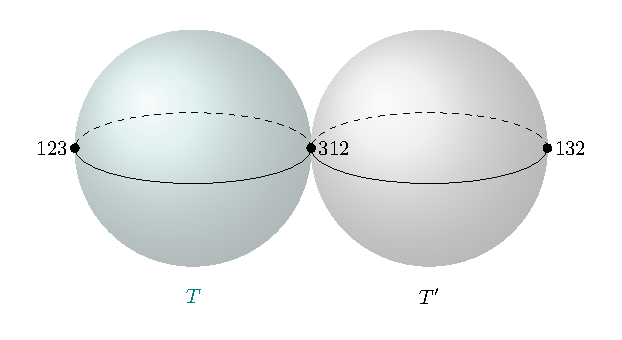
\includegraphics[width=0.75\linewidth]{./fig_springer_fiber.pdf}
        \caption{Springer Fiber $\mathcal{B}_x$}
    \end{figure}
\end{example}

\subsection{Symplectic Duality}

In \cite{braden2016quantizationsconicalsymplecticresolutions}, it is mentioned that the cotangent bundle of flag varieties forms symplectic dual pairs. In particular, we have

\begin{theorem}{\cite{braden2016quantizationsconicalsymplecticresolutions}}
    Let $G$ be a reductive algebraic group and $^LG$ be its Langlands dual. Pick Borel subgroups $B\subset G$ and $^LB\subset{^LG}$. Then $T^*(G/B)$ is symplectic dual to $T^*(^LG/^LB)$. The correspondence of fixed points is given by sending $w$ to $w^{-1}w_\circ$, and the category $\OO$ for $G$ is Koszul dual to that of $^LG$.
\end{theorem}
In particular, $T^*(G/B)$ for type $A$ is self dual.





%Consider the variety $\mathbb{C}^n/S_n$, which consists of all unordered $n$-tuples of complex numbers, alternatively viewed as the orbi-space of the symmetric group $S_n$ acting on $\mathbb{C}^n$ by permuting coordinates.

% For $x\in \mathfrak{sl}_n$, denote by $\CB{x_1, \ldots, x_n}$ the set of eigenvalues of $x$. We have $\sum_{}^{}x_i=\text{tr}\ x=0$.
% This allow us to define the map
% \[
%   \varphi:\mathfrak{sl}_n\rightarrow \CB{(x_1,\dots ,x_n)\mid \sum_{}^{}x_i=0}/S_n\subseteq \mathbb{C}^n/S_n
% \]
% by sending $x$ to the unordered tuple of eigenvalues of $x$.

% \begin{remark}
%   $\mathbb{C}^n/S_n$ is isomorphic to an $n$-dimensional vector space by identifying it with the vector space of complex polynomials in a variable $\lambda$ of degree less than or equal to $n - 1$:
%   $$
%   \psi: \mathbb{C}^{n-1}/S_n \to \mathbb{C}[\lambda]_{(n-1)} \simeq \mathbb{C}^n, \quad (x_1, \ldots, x_n) \mapsto \lambda^n - \prod_{i=1}^n (\lambda - x_i).
%   $$
% \end{remark}

% Define the \vocab{Grothendiect Simultaneous Resolution} of $\mathfrak{sl}_n$ as follows:
% \[
%   \tilde{\mathfrak{sl}}_n=\CB{(x,F)\in \mathfrak{sl}_n \times \mathfrak{B} \mid x \in \mathfrak{b}_F, \textnormal{ i.e. }x(F_i)\subseteq F_i\ \forall\ i}.
% \]
% The extra $F\in \mathfrak{B}$ can be used to order the eigenvalues of $x\in \mathfrak{sl}_n$:
% \[
%   \nu: \tilde{\mathfrak{sl}}_n \rightarrow \CB{(x_1,\dots ,x_n)\mid \sum_{}^{}x_i=0}, (x,F)\mapsto (x_1,\dots ,x_n),
% \]
% where $x_1,\dots ,x_n$ are the eigenvalues of $x$ satisfying $x(F_i/F_{i-1})=x_i(F_i/F_{i-1})$.

% Denote by $\psi:\CB{(x_1,\dots ,x_n)\mid \sum_{}^{}x_i=0}\rightarrow \CB{(x_1,\dots ,x_n)\mid \sum_{}^{}x_i=0}/S_n$ be the order forgetting map, and $\mu: \tilde{\mathfrak{sl}}_n\rightarrow \mathfrak{sl}_n$ be the first projection. We have the following commutative diagram:
% \missing{}

% We define the springer fiber of $x\in \mathfrak{sl}_n$ to be
% \[
%   \mu^{-1}(x)\simeq \mathfrak{B}_x:=\CB{F\in \mathfrak{B}\mid x(F_i)\subseteq F_i}=\CB{B\in \mathfrak{B}\mid x\in \mathfrak{B}}.
% \]

% When $x\in \mathfrak{sl}_n^{sr}$, by definition all eigenvalues are distinct. We have the following lemma:
% \begin{lemma}[lem:]{}
%   For each $x \in \mathfrak{sl}_n^{sr}$, the set $\mathcal{B}_x$ consists of $n!$ distinct flags, and there exists a canonical free action of the symmetric group $S_n$ on $\mathcal{B}_x$, making it a principal homogeneous $S_n$-space.
% \end{lemma}

% \missing{Example of Springer Fiber}

% \subsubsection{Grothendiect's Simultaneous Resolution of \mathintitle{\mathfrak{g}}}

% For general $\mathfrak{g}$, one can define the universal resolution of $\mathfrak{g}$ by
% \[
%   \tilde{\mathfrak{g}} = \{ (x, \mathfrak{b}) \in \mathfrak{g} \times \mathcal{B} \mid x \in \mathfrak{b} \}.
% \]

% Denote by $\mu:\tilde{\mathfrak{g}} \to \mathfrak{g}$ and $\pi:\tilde{\mathfrak{g}} \to \mathcal{B}$ the two coordinate projections of $\tilde{\mathfrak{g}}$.
% For any $\mathfrak{b} \in \mathcal{B}$, the fiber $\pi^{-1}(\mathfrak{b})$ consists of the vector space all elements in $\mathfrak{b}$. Thus, $\pi: \tilde{\mathfrak{g}} \to \mathcal{B}$ is a vector bundle whose fibers are the Borel subalgebras of $\mathfrak{g}$. 

% \begin{proposition}[pps:]{}
%   $\tilde{\mathfrak{g}}$ is a smooth variety with the following $G$-equivariant isomorphism for a fixe $B$:
%   \[
%     G\times _B\mathfrak{b}\xrightarrow[]{\sim}\tilde{\mathfrak{g}}, (g,x)\mapsto (gxg^{-1},g\mathfrak{b}g^{-1}).
%   \]
%   \begin{proof}
%     \missing{}
%   \end{proof}
% \end{proposition}

% $\mu:\tilde{\mathfrak{g}}\rightarrow \mathfrak{g}$ is proper as $\mathfrak{B}$ is compact. Similar as above, define the \vocab{springer fiber} of $x$ in $\mathfrak{g}$ as
% \[
%   \mu^{-1}(x)\simeq \mathfrak{B}_x=\CB{\mathfrak{b}\in \mathfrak{B}\mid x\in \mathfrak{b}}.
% \]

% In two extreme cases, where either $x = 0$ or $x$ is generic, we have

% \begin{itemize}
%   \item If $x = 0$, then $\mu^{-1}(0) = \mathcal{B}$.
%   \item If $x \in \mathfrak{g}^{sr}$, then $\# \mathcal{B}_x = \# W$.
% \end{itemize}
% In fact, we have the following:

% \begin{proposition}[pps:]{}
%   For each $x \in \mathfrak{g}^{sr}$, there exists a canonical free action of $W$ on $\mu^{-1}(x)$, making the projection $\tilde{\mathfrak{g}}^{sr} \to \mathfrak{g}^{sr}$ a principal $W$-bundle.
% \end{proposition}

% Next, we introduce an analogue of the map $v: \mathfrak{g} \to \mathbb{C}^{n-1}$ defined in the case of $\mathfrak{g} = \mathfrak{sl}_n(\mathbb{C})$. This replacement for $\mathbb{C}^{n-1}$ is the abstract Cartan subalgebra $\mathfrak{h}$. For the general case of $\mathfrak{g}$, we define the map:
% $$
% \nu: \tilde{\mathfrak{g}} \to \mathfrak{h}=\mathfrak{b}/[\mathfrak{b}, \mathfrak{b}],
% \qquad 
% (x, \mathfrak{b}) \mapsto x \mod [\mathfrak{b}, \mathfrak{b}].
% $$

% By the Chevalley Restriction Theorem, $\mathbb{C}[\mathfrak{h}]^W\simeq \mathbb{C}[\mathfrak{g}]^G$. Hence we have an embedding $\mathbb{C}[\mathfrak{h}]^W\xrightarrow[]{\simeq }\mathbb{C}[\mathfrak{g}]^G\hookrightarrow \mathbb{C}[\mathfrak{g}]$, inducing a morphism of algebraic varieties
% $\rho:\mathfrak{g}\rightarrow \mathfrak{h}/W$.

% In conclusion, we have the following commutative diagram:
% \missing{}

% \begin{remark}
%   We call $h\in \mathfrak{h}$ \vocab{regular} if it does not belong to any root hyperplanes. Equivalently, the $W$-orbit of $h$ has $\#W$ elements. For another cartan $\mathfrak{h}'$, $h'\in \mathfrak{h}'\subseteq \mathfrak{g}$ is regular if and only if the image of $h'$ in $\mathfrak{h}'\simeq \mathfrak{h}$ is regular in $\mathfrak{h}$. Denote by $\mathfrak{h}^{reg}$ the set of regular elements in $\mathfrak{h}$. Then $\mu^{-1}(\mathfrak{g}^{sr})\simeq \tilde{\mathfrak{g}}^{sr}=\nu^{-1}(\mathfrak{h}^{reg})$.
% \end{remark}

% \subsubsection{Springer Resolution}

% Denote by $\mathfrak{N}$ the nilpotent elements in $\mathfrak{g}$. It is a $\text{Ad}\ G$-stable subvariety of $\mathfrak{g}$. Moreover, it is a cone variety by a $\mathbb{C}^*$ dilation action.
% Recall the map $\mu:\tilde{\mathfrak{g}}\rightarrow \mathfrak{g}$,
% define
% \[
%   \tilde{\mathcal{N}}:=\mu^{-1}(\mathcal{N})=\CB{(x,\mathfrak{b})\in \mathcal{N}\times \mathcal{B}\mid x\in \mathfrak{b}}.
% \]
% Since we have the decomposition $\mathfrak{b}=\mathfrak{h}\oplus\mathfrak{n}$ where $\mathfrak{n}=[\mathfrak{b},\mathfrak{b}]$, $x\in \mathfrak{b}$ is nilpotent if and only if $x\in \mathfrak{n}$.
% Hence the projection $\tilde{\mathcal{N}}\rightarrow \mathcal{B}$ has fiber $\mathfrak{n}$, and 
% \[
%   \tilde{\mathcal{N}}\simeq G\times _B\mathfrak{n}.
% \]

% \missing{pps 3.2.5}

% We can extend the commutative diagram in the previous section as follows:

% \missing{example $T^*\mathbb{P}^1$}

% \begin{theorem}[thm:]{}
%   We have a natural $G$-equivariant Bundle isomorphism
%   \[
%     \tilde{\mathcal{N}}\simeq T^*\mathcal{B}.
%   \]
%   \begin{proof}
%     \missing{}
%   \end{proof}
% \end{theorem}

% \subsubsection{Moment Map and Resolution of Singularity}

% \missing{Hamiltonian action and moment map}
% \begin{corollary}[crl:]{}
%   The projection $\mu:T^*\mathcal{B}=\tilde{\mathcal{N}}\rightarrow \mathcal{N}$ is the moment map with respect to the Hamiltonian $G$-action on $T^*\mathcal{B}$ arising from the $G$-action on $\mathcal{B}$. Furthermore, $\mu$ is surjective and proper.
% \end{corollary}

% $\mu:\tilde{\mathcal{N}}\rightarrow \mathcal{N}$ is called the \vocab{Springer Resolution}.

% \begin{corollary}[crl:]{}
%   $\dim\mathcal{N}=2\dim\ \mathfrak{n}$.
% \end{corollary}

% \begin{corollary}[crl:]{}
%   $\mu^{-1}(\mathcal{N}^{reg})\simeq \tilde{\mathcal{N}}^{reg}$ is an isomorphism. Hence $\mu$ is a resolution of singularities.
% \end{corollary}

 

\section{The semismall Springer decomposition}
\label{chapter_bbdg}

We recall the form of the decomposition theorem needed for the Springer
resolution. Let $f:X\to Y$ be a proper morphism of irreducible complex
algebraic varieties, and choose a stratification
$Y=\bigsqcup_\alpha Y_\alpha$ over which $f$ is topologically locally
trivial. The morphism $f$ is \vocab{semismall} if
\[
  \dim(X\times_YX)\leq\dim X.
\]
Equivalently, for every $y\in Y_\alpha$,
\[
  2\dim f^{-1}(y)\leq\operatorname{codim}_Y(Y_\alpha).
\]
A stratum is \vocab{relevant} when equality holds.

\begin{theorem}[thm:bbdg_semismall]{\cite{Beilinson-Bernstein-Deligne1982}}
  Let $f:X\to Y$ be a semismall proper morphism with $X$ smooth and
  $Y$ irreducible. Then $Rf_*\mathbb{C}_X[\dim X]$ is a semisimple
  perverse sheaf and
  \[
    Rf_*\mathbb{C}_X[\dim X]
    \cong
    \bigoplus_{\alpha}
    \bigoplus_{L\in\operatorname{IrrLoc}(Y_\alpha)}
    IC_{\overline{Y_\alpha}}(L)\otimes V_{\alpha,L}.
  \]
  Only relevant strata occur. For $y\in Y_\alpha$, the local system
  whose isotypic multiplicity spaces are the $V_{\alpha,L}$ has fiber
  $H^{\mathrm{top}}(f^{-1}(y))$.
\end{theorem}

Now consider the Springer resolution
\[
  \pi:\widetilde{\mathcal N}\longrightarrow\mathcal N.
\]
It is semismall by the dimension calculation in
\Cref{sec:steinberg_variety}. Its strata are the nilpotent orbits, and
the monodromy on the top cohomology of a Springer fiber factors through
the component group of the centralizer. The semismall decomposition and
the Springer correspondence therefore give the following statement.

\begin{theorem}[thm:bbd_springer]{\cite{Springer1978,BM83}}
  Let $x\in\mathcal O$ and let
  \(A(x)=\pi_0(Z_G(x))\). Then
  \[
    R\pi_*\mathbb{C}_{\widetilde{\mathcal N}}
      [\dim\widetilde{\mathcal N}]
    \cong
    \bigoplus_{(\mathcal O,\chi)}
    IC_{\overline{\mathcal O}}(L_\chi)
      \otimes\rho_{\mathcal O,\chi},
  \]
  where the sum is over the pairs $(\mathcal O,\chi)$ occurring in the
  Springer correspondence, $L_\chi$ is the local system associated
  with $\chi\in\operatorname{Irr}(A(x))$, and
  $\rho_{\mathcal O,\chi}$ is the corresponding irreducible
  $W$-representation.
\end{theorem}

\subsection{Type \mathintitle{A}}

Take $G=\GL_n$. Nilpotent orbits are indexed by partitions
$\lambda\vdash n$. By \Cref{lem:centr_conn}, every centralizer
$Z_G(x)$ is connected, so $A(x)$ is trivial. Consequently, only the
constant local system occurs on each orbit. Applying the
$T$-equivariant version of the decomposition theorem and taking
hypercohomology gives
\begin{corollary}[crl:type_A_decomposition]{}
  For the type $A$ Springer resolution,
  \[
    \HH_T^\bullet(\widetilde{\mathcal N})
    \cong
    \bigoplus_{\lambda\vdash n}
    \IH_T^\bullet(\overline{\mathcal O}_\lambda)
      \otimes\Htop(\BB_\lambda).
  \]
\end{corollary}

Finally, Lusztig identifies the grading on the intersection-cohomology
factor with Kostka--Foulkes polynomials.
\begin{theorem}[thm:IH_kostka]{\cite{lusztig1981green}}
  For $x\in\mathcal O_\mu$, the Poincar\'e polynomial of the stalk of
  $IC_{\overline{\mathcal O_\lambda}}$ at $x$ is
  \[
    \sum_i q^i
      \dim\mathcal H^i(IC_{\overline{\mathcal O_\lambda}})_x
    =q^{n(\mu)-n(\lambda)}K_{\lambda,\mu}(q^{-1}),
  \]
  where
  \[
    n(\lambda)=\sum_i(i-1)\lambda_i=\dim\BB_\lambda.
  \]
  In particular,
  \[
    Q(\mathcal O_\lambda,q)
    :=\sum_iq^i\dim\IH^i(\overline{\mathcal O_\lambda})
    =q^{\binom n2-n(\lambda)}K_{\lambda,(1^n)}(q^{-1}).
  \]
\end{theorem}


\section{Main Theorem for Type $A$ Springer Resolution}
\label{chapter_main_thm}

Consider the self-dual of symplectic resolution $X = X^! = \tilde{\nilcone} \to X_0 = X_0^! = \nilcone$ given by the Springer resolution of type $A$. We would like to apply the formalism in \Cref{sec:bichar_poly} and compute the bicharacteristic polynomial.

We will prove that the bifiltration on cohomology is the direct sum of bifiltrations on the summands of \Cref{crl:type_A_decomposition}, which implies our main theorem \Cref{thm:bichar_full_flag}.

\begin{lemma}[lem:main_product_filtration]{Main Lemma}
    The bicharacteristic polynomial $T_{X,X^!}(x, y)$ equals the sum of
    \[
        x^{l(\lambda)}Q(\OO_\lambda, x^{-1})\cdot y^{l(\lambda^T)}Q(\OO_{\lambda^T}, y^{-1}) = K_{\lambda,(1)^n}(x)\cdot K_{\lambda^T,(1)^n}(y),
    \]
    over all partitions $\lambda$ of $n$.
\end{lemma}

\subsection{Category \mathintitle{\OO} and the BBD Summands}

We would like to show that the isomorphism $\misom : \HH_T(\tilde{\nilcone})_\sigma \to \HH_T(\tilde{\nilcone})_\eta$ in \Cref{eqn:m} preserves the BBD summands. To see this, we need to employ techniques from category $\mathcal{O}$. We will just briefly walk through the results we need.

By the general philosophy of \cite{braden2016quantizationsconicalsymplecticresolutions}, the pair of dominant integral characters $(\sigma, \eta)$ determines Koszul dual categories $\mathcal{O}$ and $\mathcal{O}^!$, which gives isomorphisms
\begin{equation*}
    K(\mathcal{O}) \xrightarrow{\sim} \HH_T(\tilde{\nilcone})_\sigma,
    \qquad
    K(\mathcal{O}^!) \xrightarrow{\sim} \HH_T(\tilde{\nilcone})_\eta.
\end{equation*}

The objects $P_w, L_w, S_w \in K(\mathcal{O})$ (resp. $P^!_{w^!}, L^!_{w^!}, S^!_{w^!} \in K(\mathcal{O}^!)$) are called the projective objects, simple objects, and the standard objects, indexed by the Weyl group $W$. It is known that each of these classes of objects forms a basis in the $K$-groups, and hence in the specialized cohomology. Moreover, the standard objects corresponds to the stable envelopes in our context. We have the following result compairing these objects and the BBD decomposition.

For each $w \in W$, write $\lambda_w$ the unique partition satisfying $G \cdot (\lie{n} \cap w \cdot \lie{n}) = \nilorbit_{\lambda_w}$. Recall that the ordering on the set of partitions satisfies $\nilorbit_\mu \subseteq \overline{\nilorbit_\lambda}$ if $\mu \leq \lambda$.

\begin{proposition}[prop:]{}
    The span of the BBD summands $\leq \lambda$ is generated by the classes $\{ [P_w] \mid \lambda_w \leq \lambda \}$. Dually, the span of the BBD summands $\geq \lambda$ is generated by the classes $\{ [L_w] \mid \lambda_w \geq \lambda \}$.
\end{proposition}
We now choose the local polarizations $\varepsilon$ and $\varepsilon^!$. Define $\varepsilon_w = (-1)^{\ell(w)}$ and $\varepsilon^!_{w^!} = 1$ for all $w \in W$, where $\ell$ is the length function on $W$ (for type $A$, $(-1)^{\ell(w)}$ is just the sign of the permutation $w$). This choice is motivated by \cite[Remark 10.28]{braden2016quantizationsconicalsymplecticresolutions} as follows. Note that we have 
\begin{equation*}
    \misom([S_w]) = (-1)^{\ell(w)} \misom(\Stab_\varepsilon(wB)) = (-1)^{\ell(w)} \Stab_{\varepsilon^!}(w^!B) = (-1)^{\ell(w)} [S^!_{w^!}].
\end{equation*}
By the argument in \cite[Remark 10.28]{braden2016quantizationsconicalsymplecticresolutions}, we have that $\misom([L_w]) = (-1)^{\ell(w)} [P^!_{w^!}]$ and $\misom([P_w]) = (-1)^{\ell(w)} [L^!_{w^!}]$. It follows that the BBD summands $\leq \lambda$ in $\HH_T(\tilde{\nilcone})_\sigma$ is sent to the BBD summands $\geq \lambda^T$ in $\HH_T(\tilde{\nilcone})_\eta$ under the isomorphism $\misom$, and vice versa. By taking the associated graded basis, we arrived to the following result.

\begin{proposition}[prop:m_preserves_summand]{}
    The isomorphism $\misom : \HH_T(\tilde{\nilcone})_\sigma \to \HH_T(\tilde{\nilcone})_\eta$ sends the BBD summand corresponding to $\lambda$ to the BBD summand corresponding to $\lambda^T$.
\end{proposition}
    


% \begin{definition}[def:]{}
%     Let $\mathbb{F}$ be the fraction field of $\HH^\bullet_T(\pt)$. Define the intersection pairing
%     \[
%         \AB{\ ,\ }_{\mathbb{F}}:\HH^\bullet_T(X,\mathbb{C})\otimes_{\HH^\bullet_T(\pt)}\HH^\bullet_T(X)\to \mathbb{F}
%     \]
%     as the following symmetric pairing:
%     \[
%         \AB{A,B}_{\mathbb{F}}=(-1)^{\dim_\mathbb{R} X/4}
%         \sum_{x\in X^T}^{}\frac{i^*_xA\cdot i^*_xB}{\ee(T_xX)}.
%     \]
% \end{definition}

% \begin{lemma}[lem:]{\cite[Section 6.2]{braden2016quantizationsconicalsymplecticresolutions}}
%     $\AB{[S_\alpha], [S_\beta]} = \AB{[L_\alpha], [P_\beta]}=\delta_{\alpha,\beta}$.
% \end{lemma}

% In \cite[Remark 10.28]{braden2016quantizationsconicalsymplecticresolutions}, the authors defiend a pairing $\AB{\ ,\ }_{*}$ between $K_0(\OO)_\mathbb{C}$ and $K_0(\OO^!)_\mathbb{C}$ characterized by any of the following:
% \begin{alignat*}{1}
%     \AB{[S_\alpha], [S^!_\beta]}_* &= \delta_{\alpha,\beta}\\
%     \AB{[L_\alpha], [L^!_\beta]}_* &= \delta_{\alpha,\beta}\\
%     \AB{[P_\alpha], [P^!_\beta]}_* &= \delta_{\alpha,\beta},
% \end{alignat*}

% \begin{lemma}[lem:]{}
%     We have $\AB{A,B}_*=\AB{A,\mm(B)}$.
% \end{lemma}
%\todo{The key fact is that the resolution of a simple module $L_\alpha$ by standard modules $S_\beta$ has almost the same shape as the composition series of the dual projective module $P_\alpha^!$ by standard modules. }

\subsection{A Linear Algebra Lemma}

We now prove a linear algebra statement needed for the proof of the main statement. We will work on the following abstract setting.

Let $A$ and $B$ be (not necessarily commutative) algebras over $\mathbb{C}$. In what follows, we write $\otimes$, $\mathrm{Hom}$ and $\mathrm{End}$ for $\otimes_\mathbb{C}$, $\mathrm{Hom}_\mathbb{C}$ and $\mathrm{End}_\mathbb{C}$, unless a subscript is provided.

\begin{lemma}[lem:tensor_hom]{}
    Let $M$ and $M'$ be $A$-modules and $N$ and $N'$ be $B$-modules, all of finite dimension over $\mathbb{C}$. Then, the natural map
    \begin{equation*}
        \mathrm{Hom}_A(M, M') \otimes \mathrm{Hom}_B(N, N') \to \mathrm{Hom}_{A \otimes B}(M \otimes N, M' \otimes N')
    \end{equation*}
    is an isomorphism.
    \begin{proof}
        We treat both sides as subspaces of the vector space $\mathrm{Hom}(M \otimes N, M' \otimes N')$. Since an $(A \otimes B)$-module homomorphism is nothing but a linear map that is both an $A$-module homomorphism and a $B$-modules homomorphism, we have
        \begin{equation*}
            \mathrm{Hom}_{A \otimes B}(M \otimes N, M' \otimes N') = \mathrm{Hom}_A(M \otimes N, M' \otimes N') \cap \mathrm{Hom}_B(M \otimes N, M' \otimes N').
        \end{equation*}
        By the finite-dimensionality of $N$ and $N'$, we have
        \begin{equation*}
            \mathrm{Hom}_A(M \otimes N, M' \otimes N') = \mathrm{Hom}_A(M, M') \otimes \mathrm{Hom}(N, N').
        \end{equation*}
        Similarly, by the finite-dimensionality of $M$ and $M'$, we have
        \begin{equation*}
            \mathrm{Hom}_B(M \otimes N, M' \otimes N') = \mathrm{Hom}(M, M') \otimes \mathrm{Hom}_B(N, N').
        \end{equation*}
        It follows that their intersection is $\mathrm{Hom}_A(M, M') \otimes \mathrm{Hom}_B(N, N')$.
    \end{proof}
\end{lemma}

\begin{lemma}[lem:commutes_implies_split]{}
    Let $V$ and $W$ be finite-dimensional vector spaces, $M$ be a simple $A$-module and $N$ be a simple $B$-module. Let $f : V \otimes M \to W \otimes N$ be an isomorphism of vector spaces so that the $B$-action on $V \otimes M$ induced by $f$ commutes with the original $A$-action. Assume that $\dim_\mathbb{C} M = \dim_\mathbb{C} W$ and $\dim_\mathbb{C} V = \dim_\mathbb{C} N$. Then, there are isomorphisms of vector spaces $f_1 : V \to N$ and $f_2 : M \to W$ such that $f = f_1 \otimes f_2$.
    \begin{proof}
        Since the induced $B$-action on $V \otimes M$ commutes with the original $A$-action, we have an algebra homomorphism $B \to \mathrm{End}_A(V \otimes M)$. By \Cref{lem:tensor_hom} and Schur's lemma,
        \begin{equation*}
            \mathrm{End}_A(V \otimes M) \cong \mathrm{End}(V) \otimes \mathrm{End}_A(M) = \mathrm{End}(V).
        \end{equation*}
        It follows that the $B$-action on $V \otimes M$ comes from a $B$-action on $V$. Similarly, the $A$-action on $W \otimes N$ comes from an $A$-action on $W$. By \Cref{lem:tensor_hom} again, we have
        \begin{equation*}
            f \in \mathrm{Hom}_{A \otimes B}(V \otimes M, W \otimes N) = \mathrm{Hom}_A(M, W) \otimes \mathrm{Hom}_B(V, N).
        \end{equation*}
        Note that every $A$-module homomorphism from the simple $A$-module $M$ to $W$ is either zero or injective. Since $\dim_\mathbb{C} M = \dim_\mathbb{C} W$ and $f$ is an isomorphism, we must have $M \cong W$ as $A$-modules and thus $\mathrm{Hom}_A(M, W) \cong \mathbb{C}$. Similarly, $V \cong N$ as $B$-modules and $\mathrm{Hom}_B(V, N) \cong \mathbb{C}$. Our claim follows.
    \end{proof}
\end{lemma}


\subsection{Commuting Actions}

% \begin{equation} \label{eqn:M}
%     \HH^{\bullet+2d}_T(X)_\loc \otimes_\mathbb{C} \HH^\bullet_{T^!}(\mathrm{pt})_\loc \xleftarrow[\sim]{\Stab_{\sigma, \varepsilon}^X} W^{\bullet, \bullet}_\loc \xrightarrow[\sim]{\Stab_{\eta, \varepsilon^!}^{X^!}} \HH^\bullet_T(\mathrm{pt})_\loc \otimes_\mathbb{C} \HH^{\bullet+2d^!}_{T^!}(X^!)_\loc
% \end{equation}
% Since $\sigma$ and $\eta$ are generic, we can further tensor with the evaluation $\mathbb{C}[\lie{t} \times \lie{t}^!]_\loc \to \mathbb{C}$ at the point $(\sigma, \eta) \in \lie{t}_\mathrm{reg} \times \lie{t}^!_\mathrm{reg}$ .
% \begin{equation} \label{eqn:m}
%     \HH_T(X)_\sigma \xleftarrow[\sim]{\Stab_{\sigma, \varepsilon}^X} W_{\sigma, \eta} \xrightarrow[\sim]{\Stab_{\eta, \varepsilon^!}^{X^!}} \HH_{T^!}(X^!)_\eta
% \end{equation}

The isomorphism $\misom : \HH_T(\tilde{\nilcone})_\sigma \to \HH_T(\tilde{\nilcone})_\eta$ in \Cref{eqn:m} sends the left $\HBMtop(\steinberg)$-action on $\HH_T(\tilde{\nilcone})_\sigma$ to a left $\HBMtop(\steinberg)$-action on $\HH_T(\tilde{\nilcone})_\eta$, giving us two actions on the latter space.

\begin{proposition}[prop:action_commute]{}
    The two actions by $\HBMtop(\steinberg)$ on $\HH_T(\tilde{\nilcone})_\eta$ commutes with each other.
    \begin{proof}
        We show this on the level of equivariant cohomology. By localization, we can embed both $\HH_T^\bullet(\tilde{\nilcone}) \otimes_\mathbb{C} \HH^\bullet_T(\mathrm{pt})$ and $\HH^\bullet_T(\mathrm{pt}) \otimes_\mathbb{C} \HH_T^\bullet(\tilde{\nilcone})$ into $\mathbb{C}[\lie{h} \times \lie{h}]^{\oplus W}$. Denote by $\{1_w\}_{w \in W}$ (or by $\{1^!_w\}_{w \in W}$) the standard basis corresponding to the fixed points. By \Cref{lem:W_action_on_stab}, the $W$-action induced from the former is given by $w * 1_{w'} = 1_{w'w^{-1}}$. Similarly, the $W$-action induced from the latter is given by
        \begin{equation*}
            w *^! 1_{w'} = w *^! 1^!_{{w'}^{-1} w_\circ} = 1^!_{{w'}^{-1} w_\circ w^{-1}} = 1_{w_\circ w w_\circ w'},
        \end{equation*}
        where we are manipulating the equations $w^! = w^{-1} w_\circ$ and $w = (w_\circ w^{-1})^!$. Thus, the $*$-action is given by right multiplication while the $*^!$-action is given by left multiplication, hence they commute.
    \end{proof}
\end{proposition}

\subsection{Proof of the Main Theorem}

\begin{proof}[Proof of \Cref{lem:main_product_filtration}]
    Consider the restriction of $\misom$ in \Cref{eqn:m} to the summand
    \begin{equation*}
        \misom : \mathrm{IH}^\bullet(\nilorbit_\lambda) \otimes \Htop(\borel_\lambda) \to \mathrm{IH}^\bullet(\nilorbit_{\lambda^T}) \otimes \Htop(\borel_{\lambda^T}),
    \end{equation*}
    as indicated in \Cref{prop:m_preserves_summand}. Note that $\dim \Htop(\borel_\lambda)$ is given by the number of irreducible components of $\borel_\lambda$, which by \Cref{thm:irred_springer} is given by the number of tableaux of shape $\lambda$. On the other hand, $\dim \mathrm{IH}^\bullet(\nilorbit_{\lambda^T}) = K_{\lambda^T, (1)^n}(1)$ by \Cref{thm:IH_kostka}, which by definition is the number of tableaux of shape $\lambda^T$. The two numbers are the same. On the other hand, the $\HBMtop(\steinberg) \cong \mathbb{C}[W]$ acts only on $\Htop(\borel_\lambda)$ and $\Htop(\borel_{\lambda^T})$, both irreducibly due to \Cref{thm:springer_correspondence}. Finally, by \Cref{prop:action_commute}, the induced $W$-action by $\misom$ commutes with the original one. Thus, we can apply \Cref{lem:commutes_implies_split} to conclude our claim.
\end{proof}





\appendix

\bibliographystyle{alpha}
\bibliography{ref_two_variable_polynomial}

\end{document}
